
% Default to the notebook output style

    


% Inherit from the specified cell style.




    
\documentclass[11pt]{article}

    
    
    \usepackage[T1]{fontenc}
    % Nicer default font (+ math font) than Computer Modern for most use cases
    \usepackage{mathpazo}

    % Basic figure setup, for now with no caption control since it's done
    % automatically by Pandoc (which extracts ![](path) syntax from Markdown).
    \usepackage{graphicx}
    % We will generate all images so they have a width \maxwidth. This means
    % that they will get their normal width if they fit onto the page, but
    % are scaled down if they would overflow the margins.
    \makeatletter
    \def\maxwidth{\ifdim\Gin@nat@width>\linewidth\linewidth
    \else\Gin@nat@width\fi}
    \makeatother
    \let\Oldincludegraphics\includegraphics
    % Set max figure width to be 80% of text width, for now hardcoded.
    \renewcommand{\includegraphics}[1]{\Oldincludegraphics[width=.8\maxwidth]{#1}}
    % Ensure that by default, figures have no caption (until we provide a
    % proper Figure object with a Caption API and a way to capture that
    % in the conversion process - todo).
    \usepackage{caption}
    \DeclareCaptionLabelFormat{nolabel}{}
    \captionsetup{labelformat=nolabel}

    \usepackage{adjustbox} % Used to constrain images to a maximum size 
    \usepackage{xcolor} % Allow colors to be defined
    \usepackage{enumerate} % Needed for markdown enumerations to work
    \usepackage{geometry} % Used to adjust the document margins
    \usepackage{amsmath} % Equations
    \usepackage{amssymb} % Equations
    \usepackage{textcomp} % defines textquotesingle
    % Hack from http://tex.stackexchange.com/a/47451/13684:
    \AtBeginDocument{%
        \def\PYZsq{\textquotesingle}% Upright quotes in Pygmentized code
    }
    \usepackage{upquote} % Upright quotes for verbatim code
    \usepackage{eurosym} % defines \euro
    \usepackage[mathletters]{ucs} % Extended unicode (utf-8) support
    \usepackage[utf8x]{inputenc} % Allow utf-8 characters in the tex document
    \usepackage{fancyvrb} % verbatim replacement that allows latex
    \usepackage{grffile} % extends the file name processing of package graphics 
                         % to support a larger range 
    % The hyperref package gives us a pdf with properly built
    % internal navigation ('pdf bookmarks' for the table of contents,
    % internal cross-reference links, web links for URLs, etc.)
    \usepackage{hyperref}
    \usepackage{longtable} % longtable support required by pandoc >1.10
    \usepackage{booktabs}  % table support for pandoc > 1.12.2
    \usepackage[inline]{enumitem} % IRkernel/repr support (it uses the enumerate* environment)
    \usepackage[normalem]{ulem} % ulem is needed to support strikethroughs (\sout)
                                % normalem makes italics be italics, not underlines
    

    
    
    % Colors for the hyperref package
    \definecolor{urlcolor}{rgb}{0,.145,.698}
    \definecolor{linkcolor}{rgb}{.71,0.21,0.01}
    \definecolor{citecolor}{rgb}{.12,.54,.11}

    % ANSI colors
    \definecolor{ansi-black}{HTML}{3E424D}
    \definecolor{ansi-black-intense}{HTML}{282C36}
    \definecolor{ansi-red}{HTML}{E75C58}
    \definecolor{ansi-red-intense}{HTML}{B22B31}
    \definecolor{ansi-green}{HTML}{00A250}
    \definecolor{ansi-green-intense}{HTML}{007427}
    \definecolor{ansi-yellow}{HTML}{DDB62B}
    \definecolor{ansi-yellow-intense}{HTML}{B27D12}
    \definecolor{ansi-blue}{HTML}{208FFB}
    \definecolor{ansi-blue-intense}{HTML}{0065CA}
    \definecolor{ansi-magenta}{HTML}{D160C4}
    \definecolor{ansi-magenta-intense}{HTML}{A03196}
    \definecolor{ansi-cyan}{HTML}{60C6C8}
    \definecolor{ansi-cyan-intense}{HTML}{258F8F}
    \definecolor{ansi-white}{HTML}{C5C1B4}
    \definecolor{ansi-white-intense}{HTML}{A1A6B2}

    % commands and environments needed by pandoc snippets
    % extracted from the output of `pandoc -s`
    \providecommand{\tightlist}{%
      \setlength{\itemsep}{0pt}\setlength{\parskip}{0pt}}
    \DefineVerbatimEnvironment{Highlighting}{Verbatim}{commandchars=\\\{\}}
    % Add ',fontsize=\small' for more characters per line
    \newenvironment{Shaded}{}{}
    \newcommand{\KeywordTok}[1]{\textcolor[rgb]{0.00,0.44,0.13}{\textbf{{#1}}}}
    \newcommand{\DataTypeTok}[1]{\textcolor[rgb]{0.56,0.13,0.00}{{#1}}}
    \newcommand{\DecValTok}[1]{\textcolor[rgb]{0.25,0.63,0.44}{{#1}}}
    \newcommand{\BaseNTok}[1]{\textcolor[rgb]{0.25,0.63,0.44}{{#1}}}
    \newcommand{\FloatTok}[1]{\textcolor[rgb]{0.25,0.63,0.44}{{#1}}}
    \newcommand{\CharTok}[1]{\textcolor[rgb]{0.25,0.44,0.63}{{#1}}}
    \newcommand{\StringTok}[1]{\textcolor[rgb]{0.25,0.44,0.63}{{#1}}}
    \newcommand{\CommentTok}[1]{\textcolor[rgb]{0.38,0.63,0.69}{\textit{{#1}}}}
    \newcommand{\OtherTok}[1]{\textcolor[rgb]{0.00,0.44,0.13}{{#1}}}
    \newcommand{\AlertTok}[1]{\textcolor[rgb]{1.00,0.00,0.00}{\textbf{{#1}}}}
    \newcommand{\FunctionTok}[1]{\textcolor[rgb]{0.02,0.16,0.49}{{#1}}}
    \newcommand{\RegionMarkerTok}[1]{{#1}}
    \newcommand{\ErrorTok}[1]{\textcolor[rgb]{1.00,0.00,0.00}{\textbf{{#1}}}}
    \newcommand{\NormalTok}[1]{{#1}}
    
    % Additional commands for more recent versions of Pandoc
    \newcommand{\ConstantTok}[1]{\textcolor[rgb]{0.53,0.00,0.00}{{#1}}}
    \newcommand{\SpecialCharTok}[1]{\textcolor[rgb]{0.25,0.44,0.63}{{#1}}}
    \newcommand{\VerbatimStringTok}[1]{\textcolor[rgb]{0.25,0.44,0.63}{{#1}}}
    \newcommand{\SpecialStringTok}[1]{\textcolor[rgb]{0.73,0.40,0.53}{{#1}}}
    \newcommand{\ImportTok}[1]{{#1}}
    \newcommand{\DocumentationTok}[1]{\textcolor[rgb]{0.73,0.13,0.13}{\textit{{#1}}}}
    \newcommand{\AnnotationTok}[1]{\textcolor[rgb]{0.38,0.63,0.69}{\textbf{\textit{{#1}}}}}
    \newcommand{\CommentVarTok}[1]{\textcolor[rgb]{0.38,0.63,0.69}{\textbf{\textit{{#1}}}}}
    \newcommand{\VariableTok}[1]{\textcolor[rgb]{0.10,0.09,0.49}{{#1}}}
    \newcommand{\ControlFlowTok}[1]{\textcolor[rgb]{0.00,0.44,0.13}{\textbf{{#1}}}}
    \newcommand{\OperatorTok}[1]{\textcolor[rgb]{0.40,0.40,0.40}{{#1}}}
    \newcommand{\BuiltInTok}[1]{{#1}}
    \newcommand{\ExtensionTok}[1]{{#1}}
    \newcommand{\PreprocessorTok}[1]{\textcolor[rgb]{0.74,0.48,0.00}{{#1}}}
    \newcommand{\AttributeTok}[1]{\textcolor[rgb]{0.49,0.56,0.16}{{#1}}}
    \newcommand{\InformationTok}[1]{\textcolor[rgb]{0.38,0.63,0.69}{\textbf{\textit{{#1}}}}}
    \newcommand{\WarningTok}[1]{\textcolor[rgb]{0.38,0.63,0.69}{\textbf{\textit{{#1}}}}}
    
    
    % Define a nice break command that doesn't care if a line doesn't already
    % exist.
    \def\br{\hspace*{\fill} \\* }
    % Math Jax compatability definitions
    \def\gt{>}
    \def\lt{<}
    % Document parameters
    \title{demo}
    
    
    

    % Pygments definitions
    
\makeatletter
\def\PY@reset{\let\PY@it=\relax \let\PY@bf=\relax%
    \let\PY@ul=\relax \let\PY@tc=\relax%
    \let\PY@bc=\relax \let\PY@ff=\relax}
\def\PY@tok#1{\csname PY@tok@#1\endcsname}
\def\PY@toks#1+{\ifx\relax#1\empty\else%
    \PY@tok{#1}\expandafter\PY@toks\fi}
\def\PY@do#1{\PY@bc{\PY@tc{\PY@ul{%
    \PY@it{\PY@bf{\PY@ff{#1}}}}}}}
\def\PY#1#2{\PY@reset\PY@toks#1+\relax+\PY@do{#2}}

\expandafter\def\csname PY@tok@s1\endcsname{\def\PY@tc##1{\textcolor[rgb]{0.73,0.13,0.13}{##1}}}
\expandafter\def\csname PY@tok@err\endcsname{\def\PY@bc##1{\setlength{\fboxsep}{0pt}\fcolorbox[rgb]{1.00,0.00,0.00}{1,1,1}{\strut ##1}}}
\expandafter\def\csname PY@tok@gd\endcsname{\def\PY@tc##1{\textcolor[rgb]{0.63,0.00,0.00}{##1}}}
\expandafter\def\csname PY@tok@se\endcsname{\let\PY@bf=\textbf\def\PY@tc##1{\textcolor[rgb]{0.73,0.40,0.13}{##1}}}
\expandafter\def\csname PY@tok@s\endcsname{\def\PY@tc##1{\textcolor[rgb]{0.73,0.13,0.13}{##1}}}
\expandafter\def\csname PY@tok@kt\endcsname{\def\PY@tc##1{\textcolor[rgb]{0.69,0.00,0.25}{##1}}}
\expandafter\def\csname PY@tok@il\endcsname{\def\PY@tc##1{\textcolor[rgb]{0.40,0.40,0.40}{##1}}}
\expandafter\def\csname PY@tok@ch\endcsname{\let\PY@it=\textit\def\PY@tc##1{\textcolor[rgb]{0.25,0.50,0.50}{##1}}}
\expandafter\def\csname PY@tok@sr\endcsname{\def\PY@tc##1{\textcolor[rgb]{0.73,0.40,0.53}{##1}}}
\expandafter\def\csname PY@tok@no\endcsname{\def\PY@tc##1{\textcolor[rgb]{0.53,0.00,0.00}{##1}}}
\expandafter\def\csname PY@tok@mf\endcsname{\def\PY@tc##1{\textcolor[rgb]{0.40,0.40,0.40}{##1}}}
\expandafter\def\csname PY@tok@si\endcsname{\let\PY@bf=\textbf\def\PY@tc##1{\textcolor[rgb]{0.73,0.40,0.53}{##1}}}
\expandafter\def\csname PY@tok@nf\endcsname{\def\PY@tc##1{\textcolor[rgb]{0.00,0.00,1.00}{##1}}}
\expandafter\def\csname PY@tok@kp\endcsname{\def\PY@tc##1{\textcolor[rgb]{0.00,0.50,0.00}{##1}}}
\expandafter\def\csname PY@tok@bp\endcsname{\def\PY@tc##1{\textcolor[rgb]{0.00,0.50,0.00}{##1}}}
\expandafter\def\csname PY@tok@cs\endcsname{\let\PY@it=\textit\def\PY@tc##1{\textcolor[rgb]{0.25,0.50,0.50}{##1}}}
\expandafter\def\csname PY@tok@gh\endcsname{\let\PY@bf=\textbf\def\PY@tc##1{\textcolor[rgb]{0.00,0.00,0.50}{##1}}}
\expandafter\def\csname PY@tok@vm\endcsname{\def\PY@tc##1{\textcolor[rgb]{0.10,0.09,0.49}{##1}}}
\expandafter\def\csname PY@tok@nv\endcsname{\def\PY@tc##1{\textcolor[rgb]{0.10,0.09,0.49}{##1}}}
\expandafter\def\csname PY@tok@ow\endcsname{\let\PY@bf=\textbf\def\PY@tc##1{\textcolor[rgb]{0.67,0.13,1.00}{##1}}}
\expandafter\def\csname PY@tok@w\endcsname{\def\PY@tc##1{\textcolor[rgb]{0.73,0.73,0.73}{##1}}}
\expandafter\def\csname PY@tok@nc\endcsname{\let\PY@bf=\textbf\def\PY@tc##1{\textcolor[rgb]{0.00,0.00,1.00}{##1}}}
\expandafter\def\csname PY@tok@gs\endcsname{\let\PY@bf=\textbf}
\expandafter\def\csname PY@tok@nt\endcsname{\let\PY@bf=\textbf\def\PY@tc##1{\textcolor[rgb]{0.00,0.50,0.00}{##1}}}
\expandafter\def\csname PY@tok@c\endcsname{\let\PY@it=\textit\def\PY@tc##1{\textcolor[rgb]{0.25,0.50,0.50}{##1}}}
\expandafter\def\csname PY@tok@go\endcsname{\def\PY@tc##1{\textcolor[rgb]{0.53,0.53,0.53}{##1}}}
\expandafter\def\csname PY@tok@c1\endcsname{\let\PY@it=\textit\def\PY@tc##1{\textcolor[rgb]{0.25,0.50,0.50}{##1}}}
\expandafter\def\csname PY@tok@sb\endcsname{\def\PY@tc##1{\textcolor[rgb]{0.73,0.13,0.13}{##1}}}
\expandafter\def\csname PY@tok@mo\endcsname{\def\PY@tc##1{\textcolor[rgb]{0.40,0.40,0.40}{##1}}}
\expandafter\def\csname PY@tok@m\endcsname{\def\PY@tc##1{\textcolor[rgb]{0.40,0.40,0.40}{##1}}}
\expandafter\def\csname PY@tok@cm\endcsname{\let\PY@it=\textit\def\PY@tc##1{\textcolor[rgb]{0.25,0.50,0.50}{##1}}}
\expandafter\def\csname PY@tok@nl\endcsname{\def\PY@tc##1{\textcolor[rgb]{0.63,0.63,0.00}{##1}}}
\expandafter\def\csname PY@tok@sd\endcsname{\let\PY@it=\textit\def\PY@tc##1{\textcolor[rgb]{0.73,0.13,0.13}{##1}}}
\expandafter\def\csname PY@tok@kr\endcsname{\let\PY@bf=\textbf\def\PY@tc##1{\textcolor[rgb]{0.00,0.50,0.00}{##1}}}
\expandafter\def\csname PY@tok@gu\endcsname{\let\PY@bf=\textbf\def\PY@tc##1{\textcolor[rgb]{0.50,0.00,0.50}{##1}}}
\expandafter\def\csname PY@tok@sc\endcsname{\def\PY@tc##1{\textcolor[rgb]{0.73,0.13,0.13}{##1}}}
\expandafter\def\csname PY@tok@kd\endcsname{\let\PY@bf=\textbf\def\PY@tc##1{\textcolor[rgb]{0.00,0.50,0.00}{##1}}}
\expandafter\def\csname PY@tok@gi\endcsname{\def\PY@tc##1{\textcolor[rgb]{0.00,0.63,0.00}{##1}}}
\expandafter\def\csname PY@tok@sa\endcsname{\def\PY@tc##1{\textcolor[rgb]{0.73,0.13,0.13}{##1}}}
\expandafter\def\csname PY@tok@mh\endcsname{\def\PY@tc##1{\textcolor[rgb]{0.40,0.40,0.40}{##1}}}
\expandafter\def\csname PY@tok@cp\endcsname{\def\PY@tc##1{\textcolor[rgb]{0.74,0.48,0.00}{##1}}}
\expandafter\def\csname PY@tok@mi\endcsname{\def\PY@tc##1{\textcolor[rgb]{0.40,0.40,0.40}{##1}}}
\expandafter\def\csname PY@tok@gr\endcsname{\def\PY@tc##1{\textcolor[rgb]{1.00,0.00,0.00}{##1}}}
\expandafter\def\csname PY@tok@cpf\endcsname{\let\PY@it=\textit\def\PY@tc##1{\textcolor[rgb]{0.25,0.50,0.50}{##1}}}
\expandafter\def\csname PY@tok@sx\endcsname{\def\PY@tc##1{\textcolor[rgb]{0.00,0.50,0.00}{##1}}}
\expandafter\def\csname PY@tok@vi\endcsname{\def\PY@tc##1{\textcolor[rgb]{0.10,0.09,0.49}{##1}}}
\expandafter\def\csname PY@tok@ss\endcsname{\def\PY@tc##1{\textcolor[rgb]{0.10,0.09,0.49}{##1}}}
\expandafter\def\csname PY@tok@o\endcsname{\def\PY@tc##1{\textcolor[rgb]{0.40,0.40,0.40}{##1}}}
\expandafter\def\csname PY@tok@nn\endcsname{\let\PY@bf=\textbf\def\PY@tc##1{\textcolor[rgb]{0.00,0.00,1.00}{##1}}}
\expandafter\def\csname PY@tok@kc\endcsname{\let\PY@bf=\textbf\def\PY@tc##1{\textcolor[rgb]{0.00,0.50,0.00}{##1}}}
\expandafter\def\csname PY@tok@ge\endcsname{\let\PY@it=\textit}
\expandafter\def\csname PY@tok@vg\endcsname{\def\PY@tc##1{\textcolor[rgb]{0.10,0.09,0.49}{##1}}}
\expandafter\def\csname PY@tok@gt\endcsname{\def\PY@tc##1{\textcolor[rgb]{0.00,0.27,0.87}{##1}}}
\expandafter\def\csname PY@tok@vc\endcsname{\def\PY@tc##1{\textcolor[rgb]{0.10,0.09,0.49}{##1}}}
\expandafter\def\csname PY@tok@kn\endcsname{\let\PY@bf=\textbf\def\PY@tc##1{\textcolor[rgb]{0.00,0.50,0.00}{##1}}}
\expandafter\def\csname PY@tok@mb\endcsname{\def\PY@tc##1{\textcolor[rgb]{0.40,0.40,0.40}{##1}}}
\expandafter\def\csname PY@tok@k\endcsname{\let\PY@bf=\textbf\def\PY@tc##1{\textcolor[rgb]{0.00,0.50,0.00}{##1}}}
\expandafter\def\csname PY@tok@s2\endcsname{\def\PY@tc##1{\textcolor[rgb]{0.73,0.13,0.13}{##1}}}
\expandafter\def\csname PY@tok@ne\endcsname{\let\PY@bf=\textbf\def\PY@tc##1{\textcolor[rgb]{0.82,0.25,0.23}{##1}}}
\expandafter\def\csname PY@tok@ni\endcsname{\let\PY@bf=\textbf\def\PY@tc##1{\textcolor[rgb]{0.60,0.60,0.60}{##1}}}
\expandafter\def\csname PY@tok@dl\endcsname{\def\PY@tc##1{\textcolor[rgb]{0.73,0.13,0.13}{##1}}}
\expandafter\def\csname PY@tok@fm\endcsname{\def\PY@tc##1{\textcolor[rgb]{0.00,0.00,1.00}{##1}}}
\expandafter\def\csname PY@tok@sh\endcsname{\def\PY@tc##1{\textcolor[rgb]{0.73,0.13,0.13}{##1}}}
\expandafter\def\csname PY@tok@nb\endcsname{\def\PY@tc##1{\textcolor[rgb]{0.00,0.50,0.00}{##1}}}
\expandafter\def\csname PY@tok@gp\endcsname{\let\PY@bf=\textbf\def\PY@tc##1{\textcolor[rgb]{0.00,0.00,0.50}{##1}}}
\expandafter\def\csname PY@tok@nd\endcsname{\def\PY@tc##1{\textcolor[rgb]{0.67,0.13,1.00}{##1}}}
\expandafter\def\csname PY@tok@na\endcsname{\def\PY@tc##1{\textcolor[rgb]{0.49,0.56,0.16}{##1}}}

\def\PYZbs{\char`\\}
\def\PYZus{\char`\_}
\def\PYZob{\char`\{}
\def\PYZcb{\char`\}}
\def\PYZca{\char`\^}
\def\PYZam{\char`\&}
\def\PYZlt{\char`\<}
\def\PYZgt{\char`\>}
\def\PYZsh{\char`\#}
\def\PYZpc{\char`\%}
\def\PYZdl{\char`\$}
\def\PYZhy{\char`\-}
\def\PYZsq{\char`\'}
\def\PYZdq{\char`\"}
\def\PYZti{\char`\~}
% for compatibility with earlier versions
\def\PYZat{@}
\def\PYZlb{[}
\def\PYZrb{]}
\makeatother


    % Exact colors from NB
    \definecolor{incolor}{rgb}{0.0, 0.0, 0.5}
    \definecolor{outcolor}{rgb}{0.545, 0.0, 0.0}



    
    % Prevent overflowing lines due to hard-to-break entities
    \sloppy 
    % Setup hyperref package
    \hypersetup{
      breaklinks=true,  % so long urls are correctly broken across lines
      colorlinks=true,
      urlcolor=urlcolor,
      linkcolor=linkcolor,
      citecolor=citecolor,
      }
    % Slightly bigger margins than the latex defaults
    
    \geometry{verbose,tmargin=1in,bmargin=1in,lmargin=1in,rmargin=1in}
    
    

    \begin{document}
    
    
    \maketitle
    
    

    
    \section{Comparing Feed-Forward and Convolutional Neural Networks in the
Task of Classifying Poker
Hands}\label{comparing-feed-forward-and-convolutional-neural-networks-in-the-task-of-classifying-poker-hands}

    \paragraph{Introduction:}\label{introduction}

    Poker has always shown itself to be a challenging way to test one's luck
and grit against odds that are exceptionally low. There are many
different variants that slightly alter the odds. The poker variant 5
card draw has 2,598,960 different hand combinations in a standard 52
card deck. With this many possible hands it is easy to see how difficult
it could be to get even a decent hand in a single 5 card draw. The
reason that these odds do not hinder most players is that even a
terrible hand has a chance to win with a good bluff. Great human poker
players have learned when to bluff and how to tell when another player
is bluffing. In order to compete, computerized robot players must focus
on a categorical approach based on the odds and significant training.
The overall aim of our project is to discover which techniques and
neural networks performed the best at classifying poker hands.

Our team trained two different types of Neural Networks and compared
their performance in order to assess which was superior for the problem
at hand. We will be going over them and learning about them in brief in
this demo.

    \paragraph{Installation:}\label{installation}

    In the event that you are the explorative type and ended up here before
you read the readme, here are some quick steps to get going with this
interactive demo:

Step 1: Install Jupyter here -
http://jupyter.readthedocs.io/en/latest/install.html

Step 2: Install the package Treys here -
https://github.com/ihendley/treys/tree/master/treys

This will be used to handle our deck of cards and other related things.

Step 3: Make a local copy of this repo.

    \paragraph{How does this Jupyter Notebook thing
work?:}\label{how-does-this-jupyter-notebook-thing-work}

    Jupyter notebooks work almost the exact same way as a normal programming
environment, with one very big yet simple difference. In a Jupyter
Notebook everything is divided into modular cells, so you can just run
individual segments of code instead of the entire program. All you need
to do to run a cell of code is to click on it and then press
cntrl-enter.

Otherwise everything should be relatively intuitive.

    \paragraph{What is a Neural Network?:}\label{what-is-a-neural-network}

    Maureen Caudill succinctly answered this question in 1989 and explained
Neural Networks as: "...a computing system made up of a number of
simple, highly interconnected processing elements, which process
information by their dynamic state response to external inputs". -\/-
"Neural Network Primer: Part I" by Maureen Caudill, AI Expert, Feb.
1989.

Want to learn more? Visit:
http://www.explainthatstuff.com/introduction-to-neural-networks.html

    \paragraph{Data:}\label{data}

    In order to train a Neural Network you must first have a dataset to
learn from. Our dataset is available within our repository here:
https://github.com/CSCI4850/S18-team4-project/tree/master/data

It is simply every possible hand in poker.

    \paragraph{Feed-Forward Neural
Networks:}\label{feed-forward-neural-networks}

    The first type of Neural Network we trained was a Feed-Forward Neural
Network. Feed-Forward Neural Networks are a type of Neural Network where
the connections from unit to unit don't form a cycle.

If you want to learn more in-depth about Feed-Forward Networks, please
visit:
https://www.researchgate.net/publication/228394623\_A\_brief\_review\_of\_feed-forward\_neural\_networks

    \paragraph{Our Feed-Forward Neural
Network:}\label{our-feed-forward-neural-network}

    Let's look at our results! We won't be training the network in this demo
as it can take quite a long time, but images of the entire process are
provided.

    If you want to see the actual file where this was done, please head to:
https://github.com/CSCI4850/S18-team4-project/blob/master/FeedNN.ipynb

    Okay, so let's get our data and set it up in a format our network can
understand!

    \begin{figure}[htbp]
\centering
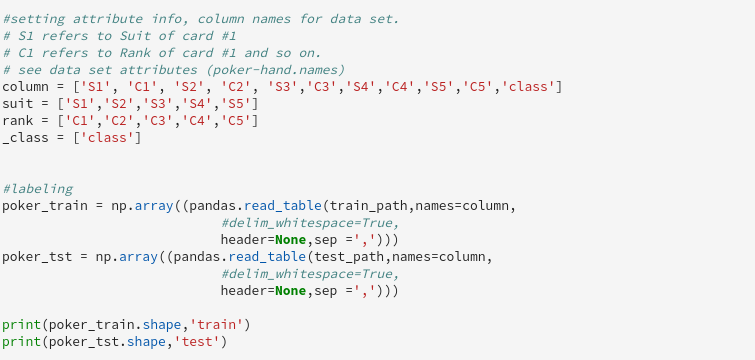
\includegraphics{setup_data_FFNN.png}
\caption{}
\end{figure}

    \begin{figure}[htbp]
\centering

\includegraphics{setup_data_FFNN_part2.png}
\caption{}
\end{figure}

    Next, we have to build our model...

    \begin{figure}[htbp]
\centering
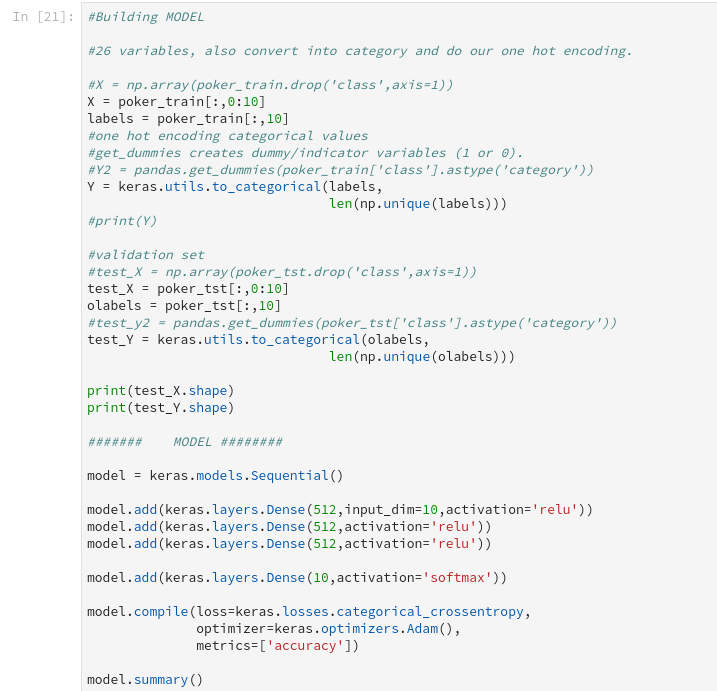
\includegraphics{build_FFNN_model.png}
\caption{}
\end{figure}

    \begin{figure}[htbp]
\centering
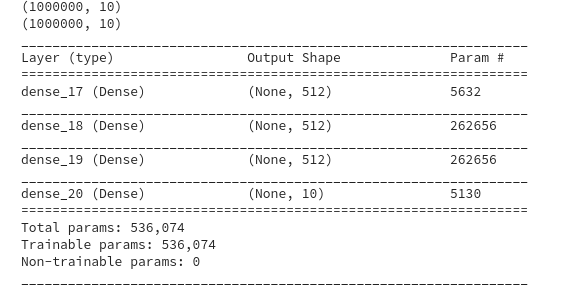
\includegraphics{build_FFNN_model_2.png}
\caption{}
\end{figure}

    Here's the part everyone always talks about, training!

    \begin{figure}[htbp]
\centering
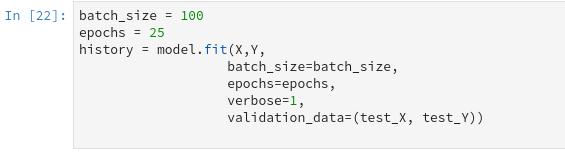
\includegraphics{train_FFNN.png}
\caption{}
\end{figure}

    \begin{figure}[htbp]
\centering
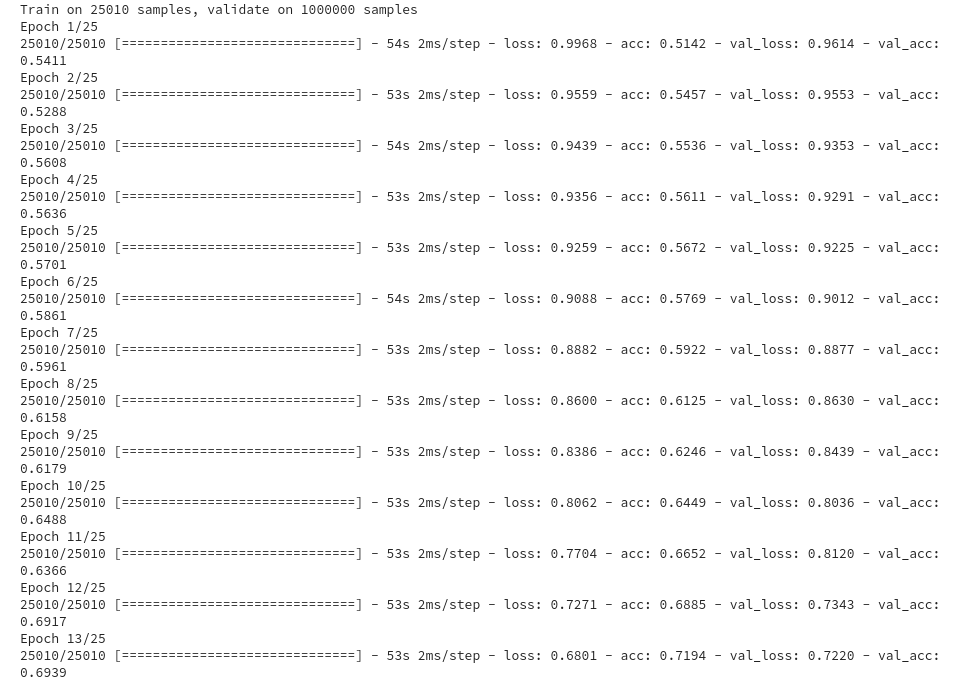
\includegraphics{train_FFNN_2.png}
\caption{}
\end{figure}

    \begin{figure}[htbp]
\centering
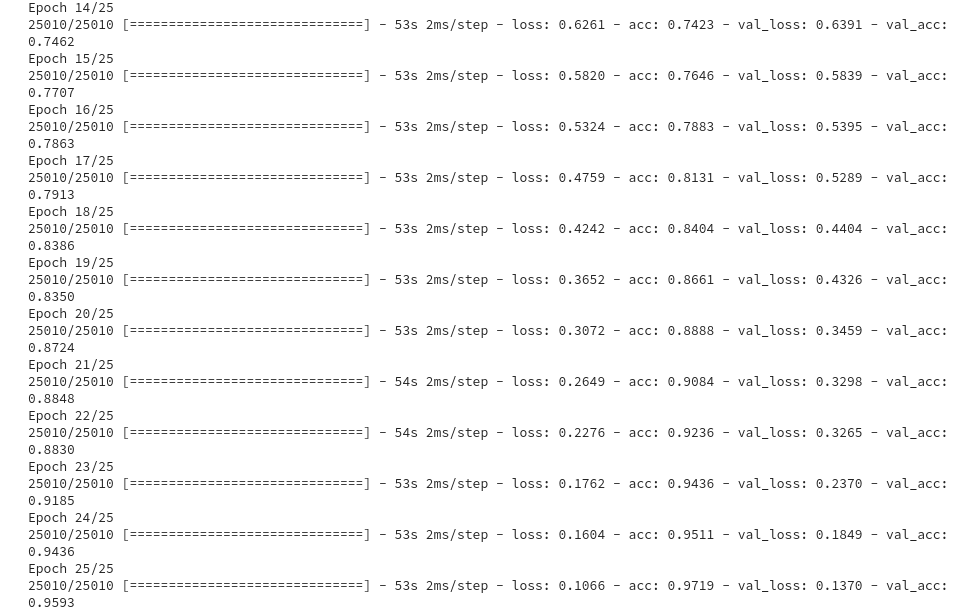
\includegraphics{train_FFNN_3.png}
\caption{}
\end{figure}

    And finally here you can see the results of our training!

    \begin{figure}[htbp]
\centering
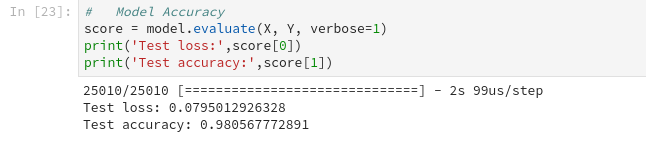
\includegraphics{results_FFNN.png}
\caption{}
\end{figure}

    \begin{figure}[htbp]
\centering
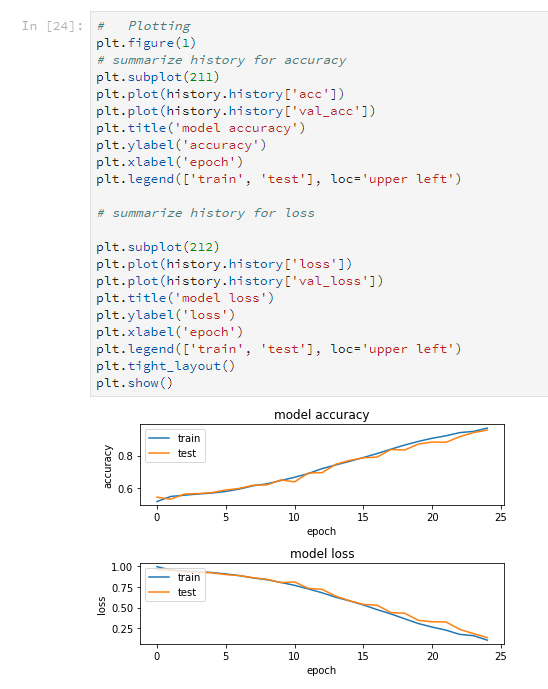
\includegraphics{ff_graph.png}
\caption{}
\end{figure}

    As you can see we got 98\% accuracy, which is really quite good!

    \paragraph{Let's play some poker against the Feed-Forward Neural
Network!
:}\label{lets-play-some-poker-against-the-feed-forward-neural-network}

    All of this work and no fun? Time to see what the above code can really
do in a game against yourself in a slightly more tangible example.

Please note that the neural network knows how to classify hands, this
means it can look at 5 cards and tell you if the hand is a high card, 2
of a kind, royal flush, etc.

All decision making based on what the neural network says the hand is
has been hard coded.

Don't worry about the following code blocks, just double click on them
one at a time and then press cntrl+enter and the game will begin!

    Setup game:

    \begin{Verbatim}[commandchars=\\\{\}]
{\color{incolor}In [{\color{incolor}143}]:} \PY{k+kn}{from} \PY{n+nn}{treys} \PY{k}{import} \PY{n}{Deck}\PY{p}{,}\PY{n}{Card}\PY{p}{,}\PY{n}{Evaluator}
          \PY{k+kn}{import} \PY{n+nn}{keras}
          \PY{k+kn}{import} \PY{n+nn}{pandas} \PY{k}{as} \PY{n+nn}{pd}
          \PY{k+kn}{import} \PY{n+nn}{numpy} \PY{k}{as} \PY{n+nn}{np}
          \PY{k+kn}{from} \PY{n+nn}{keras}\PY{n+nn}{.}\PY{n+nn}{models} \PY{k}{import} \PY{n}{load\PYZus{}model}
\end{Verbatim}


    \begin{Verbatim}[commandchars=\\\{\}]
{\color{incolor}In [{\color{incolor}147}]:} \PY{n}{deck}\PY{o}{=}\PY{n}{Deck}\PY{p}{(}\PY{p}{)}
          \PY{n}{evaluator}\PY{o}{=}\PY{n}{Evaluator}\PY{p}{(}\PY{p}{)}
          \PY{n}{trans} \PY{o}{=} \PY{p}{\PYZob{}}\PY{l+s+s1}{\PYZsq{}}\PY{l+s+s1}{Ah}\PY{l+s+s1}{\PYZsq{}}\PY{p}{:} \PY{p}{[}\PY{l+m+mi}{1}\PY{p}{,}\PY{l+m+mi}{1}\PY{p}{]}\PY{p}{,} \PY{l+s+s1}{\PYZsq{}}\PY{l+s+s1}{2h}\PY{l+s+s1}{\PYZsq{}}\PY{p}{:} \PY{p}{[}\PY{l+m+mi}{1}\PY{p}{,}\PY{l+m+mi}{2}\PY{p}{]}\PY{p}{,} \PY{l+s+s1}{\PYZsq{}}\PY{l+s+s1}{3h}\PY{l+s+s1}{\PYZsq{}}\PY{p}{:} \PY{p}{[}\PY{l+m+mi}{1}\PY{p}{,}\PY{l+m+mi}{3}\PY{p}{]}\PY{p}{,} \PY{l+s+s1}{\PYZsq{}}\PY{l+s+s1}{4h}\PY{l+s+s1}{\PYZsq{}}\PY{p}{:} \PY{p}{[}\PY{l+m+mi}{1}\PY{p}{,}\PY{l+m+mi}{4}\PY{p}{]}\PY{p}{,}\PY{l+s+s1}{\PYZsq{}}\PY{l+s+s1}{5h}\PY{l+s+s1}{\PYZsq{}}\PY{p}{:} \PY{p}{[}\PY{l+m+mi}{1}\PY{p}{,}\PY{l+m+mi}{5}\PY{p}{]}\PY{p}{,} \PY{l+s+s1}{\PYZsq{}}\PY{l+s+s1}{6h}\PY{l+s+s1}{\PYZsq{}}\PY{p}{:} \PY{p}{[}\PY{l+m+mi}{1}\PY{p}{,}\PY{l+m+mi}{6}\PY{p}{]}\PY{p}{,} \PY{l+s+s1}{\PYZsq{}}\PY{l+s+s1}{7h}\PY{l+s+s1}{\PYZsq{}}\PY{p}{:} \PY{p}{[}\PY{l+m+mi}{1}\PY{p}{,}\PY{l+m+mi}{7}\PY{p}{]}\PY{p}{,} \PY{l+s+s1}{\PYZsq{}}\PY{l+s+s1}{8h}\PY{l+s+s1}{\PYZsq{}}\PY{p}{:} \PY{p}{[}\PY{l+m+mi}{1}\PY{p}{,}\PY{l+m+mi}{8}\PY{p}{]}\PY{p}{,} \PY{l+s+s1}{\PYZsq{}}\PY{l+s+s1}{9h}\PY{l+s+s1}{\PYZsq{}}\PY{p}{:} \PY{p}{[}\PY{l+m+mi}{1}\PY{p}{,}\PY{l+m+mi}{9}\PY{p}{]}\PY{p}{,} \PY{l+s+s1}{\PYZsq{}}\PY{l+s+s1}{Th}\PY{l+s+s1}{\PYZsq{}}\PY{p}{:} \PY{p}{[}\PY{l+m+mi}{1}\PY{p}{,}\PY{l+m+mi}{10}\PY{p}{]}\PY{p}{,}\PY{l+s+s1}{\PYZsq{}}\PY{l+s+s1}{Jh}\PY{l+s+s1}{\PYZsq{}}\PY{p}{:} \PY{p}{[}\PY{l+m+mi}{1}\PY{p}{,}\PY{l+m+mi}{11}\PY{p}{]}\PY{p}{,} \PY{l+s+s1}{\PYZsq{}}\PY{l+s+s1}{Qh}\PY{l+s+s1}{\PYZsq{}}\PY{p}{:} \PY{p}{[}\PY{l+m+mi}{1}\PY{p}{,}\PY{l+m+mi}{12}\PY{p}{]}\PY{p}{,} \PY{l+s+s1}{\PYZsq{}}\PY{l+s+s1}{Kh}\PY{l+s+s1}{\PYZsq{}}\PY{p}{:} \PY{p}{[}\PY{l+m+mi}{1}\PY{p}{,}\PY{l+m+mi}{13}\PY{p}{]}\PY{p}{,}
                  \PY{l+s+s1}{\PYZsq{}}\PY{l+s+s1}{As}\PY{l+s+s1}{\PYZsq{}}\PY{p}{:} \PY{p}{[}\PY{l+m+mi}{2}\PY{p}{,}\PY{l+m+mi}{1}\PY{p}{]}\PY{p}{,} \PY{l+s+s1}{\PYZsq{}}\PY{l+s+s1}{2s}\PY{l+s+s1}{\PYZsq{}}\PY{p}{:} \PY{p}{[}\PY{l+m+mi}{2}\PY{p}{,}\PY{l+m+mi}{2}\PY{p}{]}\PY{p}{,} \PY{l+s+s1}{\PYZsq{}}\PY{l+s+s1}{3s}\PY{l+s+s1}{\PYZsq{}}\PY{p}{:} \PY{p}{[}\PY{l+m+mi}{2}\PY{p}{,}\PY{l+m+mi}{3}\PY{p}{]}\PY{p}{,} \PY{l+s+s1}{\PYZsq{}}\PY{l+s+s1}{4s}\PY{l+s+s1}{\PYZsq{}}\PY{p}{:} \PY{p}{[}\PY{l+m+mi}{2}\PY{p}{,}\PY{l+m+mi}{4}\PY{p}{]}\PY{p}{,}\PY{l+s+s1}{\PYZsq{}}\PY{l+s+s1}{5s}\PY{l+s+s1}{\PYZsq{}}\PY{p}{:} \PY{p}{[}\PY{l+m+mi}{2}\PY{p}{,}\PY{l+m+mi}{5}\PY{p}{]}\PY{p}{,} \PY{l+s+s1}{\PYZsq{}}\PY{l+s+s1}{6s}\PY{l+s+s1}{\PYZsq{}}\PY{p}{:} \PY{p}{[}\PY{l+m+mi}{2}\PY{p}{,}\PY{l+m+mi}{6}\PY{p}{]}\PY{p}{,} \PY{l+s+s1}{\PYZsq{}}\PY{l+s+s1}{7s}\PY{l+s+s1}{\PYZsq{}}\PY{p}{:} \PY{p}{[}\PY{l+m+mi}{2}\PY{p}{,}\PY{l+m+mi}{7}\PY{p}{]}\PY{p}{,} \PY{l+s+s1}{\PYZsq{}}\PY{l+s+s1}{8s}\PY{l+s+s1}{\PYZsq{}}\PY{p}{:} \PY{p}{[}\PY{l+m+mi}{2}\PY{p}{,}\PY{l+m+mi}{8}\PY{p}{]}\PY{p}{,} \PY{l+s+s1}{\PYZsq{}}\PY{l+s+s1}{9s}\PY{l+s+s1}{\PYZsq{}}\PY{p}{:} \PY{p}{[}\PY{l+m+mi}{2}\PY{p}{,}\PY{l+m+mi}{9}\PY{p}{]}\PY{p}{,} \PY{l+s+s1}{\PYZsq{}}\PY{l+s+s1}{Ts}\PY{l+s+s1}{\PYZsq{}}\PY{p}{:} \PY{p}{[}\PY{l+m+mi}{2}\PY{p}{,}\PY{l+m+mi}{10}\PY{p}{]}\PY{p}{,}\PY{l+s+s1}{\PYZsq{}}\PY{l+s+s1}{Js}\PY{l+s+s1}{\PYZsq{}}\PY{p}{:} \PY{p}{[}\PY{l+m+mi}{2}\PY{p}{,}\PY{l+m+mi}{11}\PY{p}{]}\PY{p}{,} \PY{l+s+s1}{\PYZsq{}}\PY{l+s+s1}{Qs}\PY{l+s+s1}{\PYZsq{}}\PY{p}{:} \PY{p}{[}\PY{l+m+mi}{2}\PY{p}{,}\PY{l+m+mi}{12}\PY{p}{]}\PY{p}{,} \PY{l+s+s1}{\PYZsq{}}\PY{l+s+s1}{Ks}\PY{l+s+s1}{\PYZsq{}}\PY{p}{:} \PY{p}{[}\PY{l+m+mi}{2}\PY{p}{,}\PY{l+m+mi}{13}\PY{p}{]}\PY{p}{,}
                  \PY{l+s+s1}{\PYZsq{}}\PY{l+s+s1}{Ad}\PY{l+s+s1}{\PYZsq{}}\PY{p}{:} \PY{p}{[}\PY{l+m+mi}{3}\PY{p}{,}\PY{l+m+mi}{1}\PY{p}{]}\PY{p}{,} \PY{l+s+s1}{\PYZsq{}}\PY{l+s+s1}{2d}\PY{l+s+s1}{\PYZsq{}}\PY{p}{:} \PY{p}{[}\PY{l+m+mi}{3}\PY{p}{,}\PY{l+m+mi}{2}\PY{p}{]}\PY{p}{,} \PY{l+s+s1}{\PYZsq{}}\PY{l+s+s1}{3d}\PY{l+s+s1}{\PYZsq{}}\PY{p}{:} \PY{p}{[}\PY{l+m+mi}{3}\PY{p}{,}\PY{l+m+mi}{3}\PY{p}{]}\PY{p}{,} \PY{l+s+s1}{\PYZsq{}}\PY{l+s+s1}{4d}\PY{l+s+s1}{\PYZsq{}}\PY{p}{:} \PY{p}{[}\PY{l+m+mi}{3}\PY{p}{,}\PY{l+m+mi}{4}\PY{p}{]}\PY{p}{,}\PY{l+s+s1}{\PYZsq{}}\PY{l+s+s1}{5d}\PY{l+s+s1}{\PYZsq{}}\PY{p}{:} \PY{p}{[}\PY{l+m+mi}{3}\PY{p}{,}\PY{l+m+mi}{5}\PY{p}{]}\PY{p}{,} \PY{l+s+s1}{\PYZsq{}}\PY{l+s+s1}{6d}\PY{l+s+s1}{\PYZsq{}}\PY{p}{:} \PY{p}{[}\PY{l+m+mi}{3}\PY{p}{,}\PY{l+m+mi}{6}\PY{p}{]}\PY{p}{,} \PY{l+s+s1}{\PYZsq{}}\PY{l+s+s1}{7d}\PY{l+s+s1}{\PYZsq{}}\PY{p}{:} \PY{p}{[}\PY{l+m+mi}{3}\PY{p}{,}\PY{l+m+mi}{7}\PY{p}{]}\PY{p}{,} \PY{l+s+s1}{\PYZsq{}}\PY{l+s+s1}{8d}\PY{l+s+s1}{\PYZsq{}}\PY{p}{:} \PY{p}{[}\PY{l+m+mi}{3}\PY{p}{,}\PY{l+m+mi}{8}\PY{p}{]}\PY{p}{,} \PY{l+s+s1}{\PYZsq{}}\PY{l+s+s1}{9d}\PY{l+s+s1}{\PYZsq{}}\PY{p}{:} \PY{p}{[}\PY{l+m+mi}{3}\PY{p}{,}\PY{l+m+mi}{9}\PY{p}{]}\PY{p}{,} \PY{l+s+s1}{\PYZsq{}}\PY{l+s+s1}{Td}\PY{l+s+s1}{\PYZsq{}}\PY{p}{:} \PY{p}{[}\PY{l+m+mi}{3}\PY{p}{,}\PY{l+m+mi}{10}\PY{p}{]}\PY{p}{,}\PY{l+s+s1}{\PYZsq{}}\PY{l+s+s1}{Jd}\PY{l+s+s1}{\PYZsq{}}\PY{p}{:} \PY{p}{[}\PY{l+m+mi}{3}\PY{p}{,}\PY{l+m+mi}{11}\PY{p}{]}\PY{p}{,} \PY{l+s+s1}{\PYZsq{}}\PY{l+s+s1}{Qd}\PY{l+s+s1}{\PYZsq{}}\PY{p}{:} \PY{p}{[}\PY{l+m+mi}{3}\PY{p}{,}\PY{l+m+mi}{12}\PY{p}{]}\PY{p}{,} \PY{l+s+s1}{\PYZsq{}}\PY{l+s+s1}{Kd}\PY{l+s+s1}{\PYZsq{}}\PY{p}{:} \PY{p}{[}\PY{l+m+mi}{3}\PY{p}{,}\PY{l+m+mi}{13}\PY{p}{]}\PY{p}{,}
                  \PY{l+s+s1}{\PYZsq{}}\PY{l+s+s1}{Ac}\PY{l+s+s1}{\PYZsq{}}\PY{p}{:} \PY{p}{[}\PY{l+m+mi}{4}\PY{p}{,}\PY{l+m+mi}{1}\PY{p}{]}\PY{p}{,} \PY{l+s+s1}{\PYZsq{}}\PY{l+s+s1}{2c}\PY{l+s+s1}{\PYZsq{}}\PY{p}{:} \PY{p}{[}\PY{l+m+mi}{4}\PY{p}{,}\PY{l+m+mi}{2}\PY{p}{]}\PY{p}{,} \PY{l+s+s1}{\PYZsq{}}\PY{l+s+s1}{3c}\PY{l+s+s1}{\PYZsq{}}\PY{p}{:} \PY{p}{[}\PY{l+m+mi}{4}\PY{p}{,}\PY{l+m+mi}{3}\PY{p}{]}\PY{p}{,} \PY{l+s+s1}{\PYZsq{}}\PY{l+s+s1}{4c}\PY{l+s+s1}{\PYZsq{}}\PY{p}{:} \PY{p}{[}\PY{l+m+mi}{4}\PY{p}{,}\PY{l+m+mi}{4}\PY{p}{]}\PY{p}{,}\PY{l+s+s1}{\PYZsq{}}\PY{l+s+s1}{5c}\PY{l+s+s1}{\PYZsq{}}\PY{p}{:} \PY{p}{[}\PY{l+m+mi}{4}\PY{p}{,}\PY{l+m+mi}{5}\PY{p}{]}\PY{p}{,} \PY{l+s+s1}{\PYZsq{}}\PY{l+s+s1}{6c}\PY{l+s+s1}{\PYZsq{}}\PY{p}{:} \PY{p}{[}\PY{l+m+mi}{4}\PY{p}{,}\PY{l+m+mi}{6}\PY{p}{]}\PY{p}{,} \PY{l+s+s1}{\PYZsq{}}\PY{l+s+s1}{7c}\PY{l+s+s1}{\PYZsq{}}\PY{p}{:} \PY{p}{[}\PY{l+m+mi}{4}\PY{p}{,}\PY{l+m+mi}{7}\PY{p}{]}\PY{p}{,} \PY{l+s+s1}{\PYZsq{}}\PY{l+s+s1}{8c}\PY{l+s+s1}{\PYZsq{}}\PY{p}{:} \PY{p}{[}\PY{l+m+mi}{4}\PY{p}{,}\PY{l+m+mi}{8}\PY{p}{]}\PY{p}{,} \PY{l+s+s1}{\PYZsq{}}\PY{l+s+s1}{9c}\PY{l+s+s1}{\PYZsq{}}\PY{p}{:} \PY{p}{[}\PY{l+m+mi}{4}\PY{p}{,}\PY{l+m+mi}{9}\PY{p}{]}\PY{p}{,} \PY{l+s+s1}{\PYZsq{}}\PY{l+s+s1}{Tc}\PY{l+s+s1}{\PYZsq{}}\PY{p}{:} \PY{p}{[}\PY{l+m+mi}{4}\PY{p}{,}\PY{l+m+mi}{10}\PY{p}{]}\PY{p}{,}\PY{l+s+s1}{\PYZsq{}}\PY{l+s+s1}{Jc}\PY{l+s+s1}{\PYZsq{}}\PY{p}{:} \PY{p}{[}\PY{l+m+mi}{4}\PY{p}{,}\PY{l+m+mi}{11}\PY{p}{]}\PY{p}{,} \PY{l+s+s1}{\PYZsq{}}\PY{l+s+s1}{Qc}\PY{l+s+s1}{\PYZsq{}}\PY{p}{:} \PY{p}{[}\PY{l+m+mi}{4}\PY{p}{,}\PY{l+m+mi}{12}\PY{p}{]}\PY{p}{,} \PY{l+s+s1}{\PYZsq{}}\PY{l+s+s1}{Kc}\PY{l+s+s1}{\PYZsq{}}\PY{p}{:} \PY{p}{[}\PY{l+m+mi}{4}\PY{p}{,}\PY{l+m+mi}{13}\PY{p}{]}
                  \PY{p}{\PYZcb{}} \PY{c+c1}{\PYZsh{}dict creation}
\end{Verbatim}


    Get and show initial hands:

    \begin{Verbatim}[commandchars=\\\{\}]
{\color{incolor}In [{\color{incolor}148}]:} \PY{n}{player1\PYZus{}hand}\PY{o}{=}\PY{n}{deck}\PY{o}{.}\PY{n}{draw}\PY{p}{(}\PY{l+m+mi}{5}\PY{p}{)} \PY{c+c1}{\PYZsh{}draw initial hands}
          \PY{n}{nn\PYZus{}hand}\PY{o}{=}\PY{n}{deck}\PY{o}{.}\PY{n}{draw}\PY{p}{(}\PY{l+m+mi}{5}\PY{p}{)}
          
          \PY{n}{player1\PYZus{}hand}\PY{o}{.}\PY{n}{sort}\PY{p}{(}\PY{p}{)}
          
          \PY{n+nb}{print} \PY{p}{(}\PY{l+s+s2}{\PYZdq{}}\PY{l+s+s2}{Your hand: }\PY{l+s+s2}{\PYZdq{}}\PY{p}{)}\PY{c+c1}{\PYZsh{} prints initial hands}
          \PY{n}{Card}\PY{o}{.}\PY{n}{print\PYZus{}pretty\PYZus{}cards}\PY{p}{(}\PY{n}{player1\PYZus{}hand}\PY{p}{)}
\end{Verbatim}


    \begin{Verbatim}[commandchars=\\\{\}]
Your hand: 
 [3\textcolor{ansi-red}{♥}],[4\textcolor{ansi-red}{♥}],[6\textcolor{ansi-red}{♦}],[8♣],[K♣] 

    \end{Verbatim}

    Please specify which cards you would like to discard.

Your cards are ordered 0-4 from left to right.

    \begin{Verbatim}[commandchars=\\\{\}]
{\color{incolor}In [{\color{incolor}149}]:} \PY{n}{new\PYZus{}hand}\PY{o}{=}\PY{p}{[}\PY{l+m+mi}{0}\PY{p}{,}\PY{l+m+mi}{0}\PY{p}{,}\PY{l+m+mi}{0}\PY{p}{,}\PY{l+m+mi}{0}\PY{p}{,}\PY{l+m+mi}{0}\PY{p}{]}
          \PY{n+nb}{print}\PY{p}{(}\PY{l+s+s1}{\PYZsq{}}\PY{l+s+s1}{Please enter yes or no to indicate your choice:}\PY{l+s+s1}{\PYZsq{}}\PY{p}{)}
          \PY{n+nb}{print}\PY{p}{(}\PY{l+s+s1}{\PYZsq{}}\PY{l+s+s1}{Would you like to discard your card at position 0?}\PY{l+s+s1}{\PYZsq{}}\PY{p}{,}\PY{l+s+s1}{\PYZsq{}}\PY{l+s+se}{\PYZbs{}n}\PY{l+s+s1}{\PYZsq{}}\PY{p}{)}
          \PY{n}{zero}\PY{o}{=}\PY{n+nb}{input}\PY{p}{(}\PY{p}{)}
          \PY{n+nb}{print}\PY{p}{(}\PY{l+s+s1}{\PYZsq{}}\PY{l+s+s1}{Would you like to discard your card at position 1?}\PY{l+s+s1}{\PYZsq{}}\PY{p}{,}\PY{l+s+s1}{\PYZsq{}}\PY{l+s+se}{\PYZbs{}n}\PY{l+s+s1}{\PYZsq{}}\PY{p}{)}
          \PY{n}{one}\PY{o}{=}\PY{n+nb}{input}\PY{p}{(}\PY{p}{)}
          \PY{n+nb}{print}\PY{p}{(}\PY{l+s+s1}{\PYZsq{}}\PY{l+s+s1}{Would you like to discard your card at position 2?}\PY{l+s+s1}{\PYZsq{}}\PY{p}{,}\PY{l+s+s1}{\PYZsq{}}\PY{l+s+se}{\PYZbs{}n}\PY{l+s+s1}{\PYZsq{}}\PY{p}{)}
          \PY{n}{two}\PY{o}{=}\PY{n+nb}{input}\PY{p}{(}\PY{p}{)}
          \PY{n+nb}{print}\PY{p}{(}\PY{l+s+s1}{\PYZsq{}}\PY{l+s+s1}{Would you like to discard your card at position 3?}\PY{l+s+s1}{\PYZsq{}}\PY{p}{,}\PY{l+s+s1}{\PYZsq{}}\PY{l+s+se}{\PYZbs{}n}\PY{l+s+s1}{\PYZsq{}}\PY{p}{)}
          \PY{n}{three}\PY{o}{=}\PY{n+nb}{input}\PY{p}{(}\PY{p}{)}
          \PY{n+nb}{print}\PY{p}{(}\PY{l+s+s1}{\PYZsq{}}\PY{l+s+s1}{Would you like to discard your card at position 4?}\PY{l+s+s1}{\PYZsq{}}\PY{p}{,}\PY{l+s+s1}{\PYZsq{}}\PY{l+s+se}{\PYZbs{}n}\PY{l+s+s1}{\PYZsq{}}\PY{p}{)}
          \PY{n}{four}\PY{o}{=}\PY{n+nb}{input}\PY{p}{(}\PY{p}{)}
          
          
          \PY{k}{if}\PY{p}{(}\PY{n}{zero}\PY{o}{.}\PY{n}{lower}\PY{p}{(}\PY{p}{)}\PY{o}{==}\PY{l+s+s1}{\PYZsq{}}\PY{l+s+s1}{yes}\PY{l+s+s1}{\PYZsq{}}\PY{p}{)}\PY{p}{:}
              \PY{n}{new\PYZus{}hand}\PY{p}{[}\PY{l+m+mi}{0}\PY{p}{]}\PY{o}{=}\PY{n}{deck}\PY{o}{.}\PY{n}{draw}\PY{p}{(}\PY{l+m+mi}{1}\PY{p}{)}
          \PY{k}{if}\PY{p}{(}\PY{n}{one}\PY{o}{.}\PY{n}{lower}\PY{p}{(}\PY{p}{)}\PY{o}{==}\PY{l+s+s1}{\PYZsq{}}\PY{l+s+s1}{yes}\PY{l+s+s1}{\PYZsq{}}\PY{p}{)}\PY{p}{:}
              \PY{n}{new\PYZus{}hand}\PY{p}{[}\PY{l+m+mi}{1}\PY{p}{]}\PY{o}{=}\PY{n}{deck}\PY{o}{.}\PY{n}{draw}\PY{p}{(}\PY{l+m+mi}{1}\PY{p}{)}
          \PY{k}{if}\PY{p}{(}\PY{n}{two}\PY{o}{.}\PY{n}{lower}\PY{p}{(}\PY{p}{)}\PY{o}{==}\PY{l+s+s1}{\PYZsq{}}\PY{l+s+s1}{yes}\PY{l+s+s1}{\PYZsq{}}\PY{p}{)}\PY{p}{:}
              \PY{n}{new\PYZus{}hand}\PY{p}{[}\PY{l+m+mi}{2}\PY{p}{]}\PY{o}{=}\PY{n}{deck}\PY{o}{.}\PY{n}{draw}\PY{p}{(}\PY{l+m+mi}{1}\PY{p}{)}
          \PY{k}{if}\PY{p}{(}\PY{n}{three}\PY{o}{.}\PY{n}{lower}\PY{p}{(}\PY{p}{)}\PY{o}{==}\PY{l+s+s1}{\PYZsq{}}\PY{l+s+s1}{yes}\PY{l+s+s1}{\PYZsq{}}\PY{p}{)}\PY{p}{:}
              \PY{n}{new\PYZus{}hand}\PY{p}{[}\PY{l+m+mi}{3}\PY{p}{]}\PY{o}{=}\PY{n}{deck}\PY{o}{.}\PY{n}{draw}\PY{p}{(}\PY{l+m+mi}{1}\PY{p}{)}
          \PY{k}{if}\PY{p}{(}\PY{n}{four}\PY{o}{.}\PY{n}{lower}\PY{p}{(}\PY{p}{)}\PY{o}{==}\PY{l+s+s1}{\PYZsq{}}\PY{l+s+s1}{yes}\PY{l+s+s1}{\PYZsq{}}\PY{p}{)}\PY{p}{:}
              \PY{n}{new\PYZus{}hand}\PY{p}{[}\PY{l+m+mi}{4}\PY{p}{]}\PY{o}{=}\PY{n}{deck}\PY{o}{.}\PY{n}{draw}\PY{p}{(}\PY{l+m+mi}{1}\PY{p}{)}
          
          \PY{k}{for} \PY{n}{i} \PY{o+ow}{in} \PY{n+nb}{range}\PY{p}{(}\PY{l+m+mi}{0}\PY{p}{,}\PY{l+m+mi}{5}\PY{p}{)}\PY{p}{:}
              \PY{k}{if}\PY{p}{(}\PY{n}{new\PYZus{}hand}\PY{p}{[}\PY{n}{i}\PY{p}{]}\PY{o}{!=}\PY{l+m+mi}{0}\PY{p}{)}\PY{p}{:}
                  \PY{n}{player1\PYZus{}hand}\PY{p}{[}\PY{n}{i}\PY{p}{]}\PY{o}{=}\PY{n}{new\PYZus{}hand}\PY{p}{[}\PY{n}{i}\PY{p}{]}        
          
          \PY{n+nb}{print}\PY{p}{(}\PY{l+s+s2}{\PYZdq{}}\PY{l+s+s2}{Your current hand is:}\PY{l+s+s2}{\PYZdq{}} \PY{p}{,}\PY{l+s+s1}{\PYZsq{}}\PY{l+s+se}{\PYZbs{}n}\PY{l+s+s1}{\PYZsq{}}\PY{p}{)}
          \PY{n}{Card}\PY{o}{.}\PY{n}{print\PYZus{}pretty\PYZus{}cards}\PY{p}{(}\PY{n}{player1\PYZus{}hand}\PY{p}{)}
\end{Verbatim}


    \begin{Verbatim}[commandchars=\\\{\}]
Please enter yes or no to indicate your choice:
Would you like to discard your card at position 0? 

Would you like to discard your card at position 1? 

Would you like to discard your card at position 2? 

Would you like to discard your card at position 3? 

Would you like to discard your card at position 4? 

Your current hand is: 

 [K\textcolor{ansi-red}{♥}],[2\textcolor{ansi-red}{♥}],[Q\textcolor{ansi-red}{♦}],[Q♠],[3♠] 

    \end{Verbatim}

    \paragraph{Note: You might want to wait \textasciitilde{}20 seconds for
the code in this next cell to
finish...}\label{note-you-might-want-to-wait-20-seconds-for-the-code-in-this-next-cell-to-finish...}

    \begin{Verbatim}[commandchars=\\\{\}]
{\color{incolor}In [{\color{incolor}150}]:} \PY{c+c1}{\PYZsh{}determine what the NN thinks of the hand}
          \PY{n}{hand\PYZus{}for\PYZus{}nn}\PY{o}{=}\PY{p}{[}\PY{p}{]}
          \PY{k}{for} \PY{n}{i} \PY{o+ow}{in} \PY{n+nb}{range}\PY{p}{(}\PY{l+m+mi}{0}\PY{p}{,}\PY{l+m+mi}{5}\PY{p}{)}\PY{p}{:}
              \PY{n}{hand\PYZus{}for\PYZus{}nn}\PY{o}{=}\PY{p}{(}\PY{n}{hand\PYZus{}for\PYZus{}nn}\PY{o}{+}\PY{n}{trans}\PY{p}{[}\PY{n}{Card}\PY{o}{.}\PY{n}{int\PYZus{}to\PYZus{}str}\PY{p}{(}\PY{n}{nn\PYZus{}hand}\PY{p}{[}\PY{n}{i}\PY{p}{]}\PY{p}{)}\PY{p}{]}\PY{p}{)}
          
              
              
          \PY{n}{model} \PY{o}{=} \PY{n}{load\PYZus{}model}\PY{p}{(}\PY{l+s+s1}{\PYZsq{}}\PY{l+s+s1}{demo/ffbnn.h5}\PY{l+s+s1}{\PYZsq{}}\PY{p}{)} \PY{c+c1}{\PYZsh{}ffbnn.h5 is feed forward NN}
          
          \PY{n}{handarray} \PY{o}{=} \PY{n}{np}\PY{o}{.}\PY{n}{array}\PY{p}{(}\PY{p}{[}\PY{n}{hand\PYZus{}for\PYZus{}nn}\PY{p}{]}\PY{p}{)} \PY{c+c1}{\PYZsh{}convert hand to np array for input}
          
          \PY{n}{preds} \PY{o}{=} \PY{n}{model}\PY{o}{.}\PY{n}{predict}\PY{p}{(}\PY{n}{handarray}\PY{p}{)} \PY{c+c1}{\PYZsh{}calculates probabilities of each class from NN}
          
          \PY{n}{label}\PY{o}{=}\PY{n}{np}\PY{o}{.}\PY{n}{argmax}\PY{p}{(}\PY{n}{preds}\PY{p}{)}
          
          \PY{c+c1}{\PYZsh{}if nothing in hand}
          \PY{k}{if} \PY{p}{(}\PY{n}{label}\PY{o}{==}\PY{l+m+mi}{0}\PY{p}{)}\PY{p}{:}
              
              \PY{n}{new\PYZus{}hand}\PY{o}{=}\PY{n}{deck}\PY{o}{.}\PY{n}{draw}\PY{p}{(}\PY{l+m+mi}{5}\PY{p}{)}\PY{c+c1}{\PYZsh{}draw 5 new cards}
              
              
          \PY{c+c1}{\PYZsh{}if one pair}
          \PY{k}{if} \PY{p}{(}\PY{n}{label}\PY{o}{==}\PY{l+m+mi}{1}\PY{p}{)}\PY{p}{:}
              \PY{n}{nn\PYZus{}hand}\PY{o}{.}\PY{n}{sort}\PY{p}{(}\PY{p}{)} \PY{c+c1}{\PYZsh{}sort arr by val}
              
              
              \PY{n}{cards\PYZus{}to\PYZus{}keep}\PY{o}{=}\PY{p}{[}\PY{l+m+mi}{0}\PY{p}{,}\PY{l+m+mi}{0}\PY{p}{]} \PY{c+c1}{\PYZsh{}array where will store the cards from hand to keep, init as strings for testing}
              \PY{n}{new\PYZus{}hand}\PY{o}{=}\PY{p}{[}\PY{l+m+mi}{0}\PY{p}{,}\PY{l+m+mi}{0}\PY{p}{]} \PY{c+c1}{\PYZsh{}actual arr where cards will be stored as their int encodings}
              \PY{n}{count}\PY{o}{=}\PY{l+m+mi}{2}
              \PY{k}{for} \PY{n}{i} \PY{o+ow}{in} \PY{n+nb}{range}\PY{p}{(}\PY{l+m+mi}{0}\PY{p}{,}\PY{l+m+mi}{4}\PY{p}{)}\PY{p}{:}
                  \PY{n}{current}\PY{o}{=}\PY{n}{Card}\PY{o}{.}\PY{n}{int\PYZus{}to\PYZus{}str}\PY{p}{(}\PY{n}{nn\PYZus{}hand}\PY{p}{[}\PY{n}{i}\PY{p}{]}\PY{p}{)} \PY{c+c1}{\PYZsh{}get card as str}
                  \PY{n}{current\PYZus{}num}\PY{o}{=}\PY{n}{nn\PYZus{}hand}\PY{p}{[}\PY{n}{i}\PY{p}{]}
                  \PY{k}{for} \PY{n}{x} \PY{o+ow}{in} \PY{n+nb}{range}\PY{p}{(}\PY{l+m+mi}{0}\PY{p}{,}\PY{l+m+mi}{5}\PY{p}{)}\PY{p}{:}
                      \PY{k}{if} \PY{p}{(}\PY{n}{x}\PY{o}{!=}\PY{n}{i}\PY{p}{)}\PY{p}{:} \PY{c+c1}{\PYZsh{}if we\PYZsq{}re not on the card we are checking for a match for}
                          \PY{n}{check}\PY{o}{=}\PY{n}{Card}\PY{o}{.}\PY{n}{int\PYZus{}to\PYZus{}str}\PY{p}{(}\PY{n}{nn\PYZus{}hand}\PY{p}{[}\PY{n}{x}\PY{p}{]}\PY{p}{)} \PY{c+c1}{\PYZsh{}get card to check against current}
                          \PY{n}{check\PYZus{}num}\PY{o}{=}\PY{n}{nn\PYZus{}hand}\PY{p}{[}\PY{n}{x}\PY{p}{]}
                          \PY{k}{if}\PY{p}{(}\PY{n}{check}\PY{p}{[}\PY{l+m+mi}{0}\PY{p}{]}\PY{o}{==}\PY{n}{current}\PY{p}{[}\PY{l+m+mi}{0}\PY{p}{]}\PY{p}{)}\PY{p}{:} \PY{c+c1}{\PYZsh{}if the cards have the same value aka are a pair}
                              \PY{n}{cards\PYZus{}to\PYZus{}keep}\PY{p}{[}\PY{l+m+mi}{0}\PY{p}{]}\PY{o}{=}\PY{n}{check}
                              \PY{n}{cards\PYZus{}to\PYZus{}keep}\PY{p}{[}\PY{l+m+mi}{1}\PY{p}{]}\PY{o}{=}\PY{n}{current}
                              
                              \PY{n}{new\PYZus{}hand}\PY{p}{[}\PY{l+m+mi}{0}\PY{p}{]}\PY{o}{=}\PY{n}{check\PYZus{}num} 
                              \PY{n}{new\PYZus{}hand}\PY{p}{[}\PY{l+m+mi}{1}\PY{p}{]}\PY{o}{=}\PY{n}{current\PYZus{}num}
                              
                              
                              
              \PY{n}{draw\PYZus{}3}\PY{o}{=}\PY{n}{deck}\PY{o}{.}\PY{n}{draw}\PY{p}{(}\PY{l+m+mi}{3}\PY{p}{)}\PY{c+c1}{\PYZsh{}draw 3 new cards}
              \PY{n}{new\PYZus{}hand}\PY{o}{=}\PY{n}{new\PYZus{}hand}\PY{o}{+}\PY{n}{draw\PYZus{}3} \PY{c+c1}{\PYZsh{}add the 3 new cards to the hand, keeping the pairs}
                              
              \PY{n}{Card}\PY{o}{.}\PY{n}{print\PYZus{}pretty\PYZus{}cards}\PY{p}{(}\PY{n}{new\PYZus{}hand}\PY{p}{)}
              \PY{c+c1}{\PYZsh{}for y in range(0,5):}
               \PY{c+c1}{\PYZsh{}   print(Card.int\PYZus{}to\PYZus{}str(new\PYZus{}hand[y]))}
                          
                      
          \PY{k}{if} \PY{p}{(}\PY{n}{label}\PY{o}{==}\PY{l+m+mi}{2}\PY{p}{)}\PY{p}{:} \PY{c+c1}{\PYZsh{}two pairs}
              
              
             
              
              \PY{n}{nn\PYZus{}hand}\PY{o}{.}\PY{n}{sort}\PY{p}{(}\PY{p}{)} \PY{c+c1}{\PYZsh{}sort arr by val}
              
              \PY{n}{cards\PYZus{}to\PYZus{}keep}\PY{o}{=}\PY{p}{[}\PY{l+m+mi}{0}\PY{p}{,}\PY{l+m+mi}{0}\PY{p}{,}\PY{l+m+mi}{0}\PY{p}{,}\PY{l+m+mi}{0}\PY{p}{]} \PY{c+c1}{\PYZsh{}array where will store the cards from hand to keep, init as strings for testing}
              \PY{n}{new\PYZus{}hand}\PY{o}{=}\PY{p}{[}\PY{l+m+mi}{0}\PY{p}{,}\PY{l+m+mi}{0}\PY{p}{,}\PY{l+m+mi}{0}\PY{p}{,}\PY{l+m+mi}{0}\PY{p}{]} \PY{c+c1}{\PYZsh{}actual arr where cards will be stored as their int encodings}
              \PY{n}{count}\PY{o}{=}\PY{l+m+mi}{0}
              \PY{n}{has\PYZus{}1\PYZus{}pair}\PY{o}{=}\PY{l+m+mi}{0}
              \PY{k}{for} \PY{n}{i} \PY{o+ow}{in} \PY{n+nb}{range}\PY{p}{(}\PY{l+m+mi}{0}\PY{p}{,}\PY{l+m+mi}{4}\PY{p}{)}\PY{p}{:}
                  \PY{n}{current}\PY{o}{=}\PY{n}{Card}\PY{o}{.}\PY{n}{int\PYZus{}to\PYZus{}str}\PY{p}{(}\PY{n}{nn\PYZus{}hand}\PY{p}{[}\PY{n}{i}\PY{p}{]}\PY{p}{)} \PY{c+c1}{\PYZsh{}get card as str}
                  \PY{n}{current\PYZus{}num}\PY{o}{=}\PY{n}{nn\PYZus{}hand}\PY{p}{[}\PY{n}{i}\PY{p}{]}
                  \PY{k}{if}\PY{p}{(}\PY{n}{i}\PY{o}{==}\PY{l+m+mi}{4}\PY{p}{)}\PY{p}{:}
                      \PY{k}{break}
                  \PY{k}{for} \PY{n}{x} \PY{o+ow}{in} \PY{n+nb}{range}\PY{p}{(}\PY{l+m+mi}{0}\PY{p}{,}\PY{l+m+mi}{5}\PY{p}{)}\PY{p}{:}
                      \PY{k}{if} \PY{p}{(}\PY{n}{x}\PY{o}{!=}\PY{n}{i}\PY{p}{)}\PY{p}{:} \PY{c+c1}{\PYZsh{}if we\PYZsq{}re not on the card we are checking for a match for}
                          \PY{n}{check}\PY{o}{=}\PY{n}{Card}\PY{o}{.}\PY{n}{int\PYZus{}to\PYZus{}str}\PY{p}{(}\PY{n}{nn\PYZus{}hand}\PY{p}{[}\PY{n}{x}\PY{p}{]}\PY{p}{)} \PY{c+c1}{\PYZsh{}get card to check against current}
                          \PY{n}{check\PYZus{}num}\PY{o}{=}\PY{n}{nn\PYZus{}hand}\PY{p}{[}\PY{n}{x}\PY{p}{]}
                          \PY{k}{if}\PY{p}{(}\PY{n}{check}\PY{p}{[}\PY{l+m+mi}{0}\PY{p}{]}\PY{o}{==}\PY{n}{current}\PY{p}{[}\PY{l+m+mi}{0}\PY{p}{]} \PY{o+ow}{and} \PY{p}{(}\PY{n}{check\PYZus{}num}\PY{o}{!=}\PY{n}{new\PYZus{}hand}\PY{p}{[}\PY{l+m+mi}{0}\PY{p}{]} \PY{o+ow}{and} \PY{n}{check\PYZus{}num}\PY{o}{!=}\PY{n}{new\PYZus{}hand}\PY{p}{[}\PY{l+m+mi}{1}\PY{p}{]}\PY{p}{)}\PY{p}{)}\PY{p}{:} \PY{c+c1}{\PYZsh{}if the cards have the same value aka are a pair }
                              \PY{k}{for} \PY{n}{y} \PY{o+ow}{in} \PY{n+nb}{range}\PY{p}{(}\PY{l+m+mi}{0}\PY{p}{,}\PY{l+m+mi}{4}\PY{p}{)}\PY{p}{:}
                                  \PY{k}{if} \PY{p}{(}\PY{n}{check\PYZus{}num} \PY{o+ow}{not} \PY{o+ow}{in} \PY{n}{new\PYZus{}hand}\PY{p}{)}\PY{p}{:} \PY{c+c1}{\PYZsh{}man python is nice}
                                      \PY{n}{cards\PYZus{}to\PYZus{}keep}\PY{p}{[}\PY{n}{count}\PY{p}{]}\PY{o}{=}\PY{n}{check}
                                      \PY{n}{new\PYZus{}hand}\PY{p}{[}\PY{n}{count}\PY{p}{]}\PY{o}{=}\PY{n}{check\PYZus{}num}
                                      \PY{n}{count}\PY{o}{+}\PY{o}{=}\PY{l+m+mi}{1}
                                      \PY{n}{cards\PYZus{}to\PYZus{}keep}\PY{p}{[}\PY{n}{count}\PY{p}{]}\PY{o}{=}\PY{n}{current}
                                      \PY{n}{new\PYZus{}hand}\PY{p}{[}\PY{n}{count}\PY{p}{]}\PY{o}{=}\PY{n}{current\PYZus{}num}
                                      \PY{n}{count}\PY{o}{+}\PY{o}{=}\PY{l+m+mi}{1}
                                      \PY{c+c1}{\PYZsh{}print(len(new\PYZus{}hand))}
                              
                             
              \PY{n}{draw\PYZus{}1}\PY{o}{=}\PY{n}{deck}\PY{o}{.}\PY{n}{draw}\PY{p}{(}\PY{l+m+mi}{1}\PY{p}{)}\PY{c+c1}{\PYZsh{}draw 1 new card}
              \PY{n}{drawn}\PY{o}{=}\PY{p}{[}\PY{n}{draw\PYZus{}1}\PY{p}{]}
              \PY{n}{new\PYZus{}hand}\PY{o}{=}\PY{n}{new\PYZus{}hand}\PY{o}{+}\PY{n}{drawn} \PY{c+c1}{\PYZsh{}add the new card to the hand, keeping the pairs}
                          
              
              
          \PY{k}{if} \PY{p}{(}\PY{n}{label}\PY{o}{==}\PY{l+m+mi}{3}\PY{p}{)}\PY{p}{:} \PY{c+c1}{\PYZsh{}three of a kind}
              \PY{n}{nn\PYZus{}hand}\PY{o}{.}\PY{n}{sort}\PY{p}{(}\PY{p}{)} \PY{c+c1}{\PYZsh{}sort arr by val}
             
              \PY{n}{cards\PYZus{}to\PYZus{}keep}\PY{o}{=}\PY{p}{[}\PY{l+m+mi}{0}\PY{p}{,}\PY{l+m+mi}{0}\PY{p}{,}\PY{l+m+mi}{0}\PY{p}{]} \PY{c+c1}{\PYZsh{}array where will store the cards from hand to keep, init as strings for testing}
              \PY{n}{new\PYZus{}hand}\PY{o}{=}\PY{p}{[}\PY{l+m+mi}{0}\PY{p}{,}\PY{l+m+mi}{0}\PY{p}{,}\PY{l+m+mi}{0}\PY{p}{]} \PY{c+c1}{\PYZsh{}actual arr where cards will be stored as their int encodings}
              \PY{n}{count}\PY{o}{=}\PY{l+m+mi}{0}
              \PY{k}{for} \PY{n}{i} \PY{o+ow}{in} \PY{n+nb}{range}\PY{p}{(}\PY{l+m+mi}{0}\PY{p}{,}\PY{l+m+mi}{4}\PY{p}{)}\PY{p}{:}
                  \PY{n}{current}\PY{o}{=}\PY{n}{Card}\PY{o}{.}\PY{n}{int\PYZus{}to\PYZus{}str}\PY{p}{(}\PY{n}{nn\PYZus{}hand}\PY{p}{[}\PY{n}{i}\PY{p}{]}\PY{p}{)} \PY{c+c1}{\PYZsh{}get card as str}
                  \PY{n}{current\PYZus{}num}\PY{o}{=}\PY{n}{nn\PYZus{}hand}\PY{p}{[}\PY{n}{i}\PY{p}{]}
                  \PY{k}{for} \PY{n}{x} \PY{o+ow}{in} \PY{n+nb}{range}\PY{p}{(}\PY{l+m+mi}{0}\PY{p}{,}\PY{l+m+mi}{4}\PY{p}{)}\PY{p}{:}
                      \PY{k}{if} \PY{p}{(}\PY{n}{x}\PY{o}{!=}\PY{n}{i}\PY{p}{)}\PY{p}{:} \PY{c+c1}{\PYZsh{}if we\PYZsq{}re not on the card we are checking for a match for}
                          \PY{n}{check}\PY{o}{=}\PY{n}{Card}\PY{o}{.}\PY{n}{int\PYZus{}to\PYZus{}str}\PY{p}{(}\PY{n}{nn\PYZus{}hand}\PY{p}{[}\PY{n}{x}\PY{p}{]}\PY{p}{)} \PY{c+c1}{\PYZsh{}get card to check against current}
                          \PY{n}{check\PYZus{}num}\PY{o}{=}\PY{n}{nn\PYZus{}hand}\PY{p}{[}\PY{n}{x}\PY{p}{]}
                          \PY{k}{if}\PY{p}{(}\PY{n}{check}\PY{p}{[}\PY{l+m+mi}{0}\PY{p}{]}\PY{o}{==}\PY{n}{current}\PY{p}{[}\PY{l+m+mi}{0}\PY{p}{]}\PY{p}{)}\PY{p}{:} \PY{c+c1}{\PYZsh{}if the cards have the same value aka are a pair}
                              \PY{n}{cards\PYZus{}to\PYZus{}keep}\PY{p}{[}\PY{l+m+mi}{0}\PY{p}{]}\PY{o}{=}\PY{n}{check}
                              \PY{n}{cards\PYZus{}to\PYZus{}keep}\PY{p}{[}\PY{l+m+mi}{1}\PY{p}{]}\PY{o}{=}\PY{n}{current}
                              
                              \PY{n}{new\PYZus{}hand}\PY{p}{[}\PY{l+m+mi}{0}\PY{p}{]}\PY{o}{=}\PY{n}{check\PYZus{}num} 
                              \PY{n}{new\PYZus{}hand}\PY{p}{[}\PY{l+m+mi}{1}\PY{p}{]}\PY{o}{=}\PY{n}{current\PYZus{}num}
                             
                              
                              \PY{c+c1}{\PYZsh{}find third card}
                              \PY{k}{for} \PY{n}{y} \PY{o+ow}{in} \PY{n+nb}{range}\PY{p}{(}\PY{l+m+mi}{0}\PY{p}{,}\PY{l+m+mi}{5}\PY{p}{)}\PY{p}{:}
                                  \PY{n}{check2}\PY{o}{=}\PY{n}{Card}\PY{o}{.}\PY{n}{int\PYZus{}to\PYZus{}str}\PY{p}{(}\PY{n}{nn\PYZus{}hand}\PY{p}{[}\PY{n}{y}\PY{p}{]}\PY{p}{)}
                                  \PY{k}{if}\PY{p}{(}\PY{n}{check2}\PY{p}{[}\PY{l+m+mi}{0}\PY{p}{]}\PY{o}{==}\PY{n}{current}\PY{p}{[}\PY{l+m+mi}{0}\PY{p}{]} \PY{o+ow}{and} \PY{p}{(}\PY{n}{check2}\PY{p}{[}\PY{l+m+mi}{1}\PY{p}{]}\PY{o}{!=}\PY{n}{check}\PY{p}{[}\PY{l+m+mi}{1}\PY{p}{]} \PY{o+ow}{and} \PY{n}{check2}\PY{p}{[}\PY{l+m+mi}{1}\PY{p}{]}\PY{o}{!=}\PY{n}{current}\PY{p}{[}\PY{l+m+mi}{1}\PY{p}{]}\PY{p}{)}\PY{p}{)}\PY{p}{:} \PY{c+c1}{\PYZsh{}if card is same val as other 2 and not already in the list to keep \PYZsh{}can also use not in list}
                                      \PY{n}{store}\PY{o}{=}\PY{n}{nn\PYZus{}hand}\PY{p}{[}\PY{n}{y}\PY{p}{]}
                                      
                                      \PY{n}{new\PYZus{}hand}\PY{p}{[}\PY{l+m+mi}{2}\PY{p}{]}\PY{o}{=}\PY{n}{new\PYZus{}hand}\PY{p}{[}\PY{l+m+mi}{1}\PY{p}{]}
                                      \PY{n}{new\PYZus{}hand}\PY{p}{[}\PY{l+m+mi}{1}\PY{p}{]}\PY{o}{=}\PY{n}{store}
                                      \PY{n}{cards\PYZus{}to\PYZus{}keep}\PY{p}{[}\PY{l+m+mi}{2}\PY{p}{]}\PY{o}{=}\PY{n}{check2}
                              
                              
                             
              \PY{n}{draw\PYZus{}2}\PY{o}{=}\PY{n}{deck}\PY{o}{.}\PY{n}{draw}\PY{p}{(}\PY{l+m+mi}{2}\PY{p}{)}\PY{c+c1}{\PYZsh{}draw 2 new cards}
              \PY{n}{new\PYZus{}hand}\PY{o}{=}\PY{n}{new\PYZus{}hand}\PY{o}{+}\PY{n}{draw\PYZus{}2} \PY{c+c1}{\PYZsh{}add the 2 new cards to the hand, keeping the pairs}
              
             
              
          
          \PY{k}{if}\PY{p}{(}\PY{n}{label}\PY{o}{\PYZgt{}}\PY{l+m+mi}{3}\PY{p}{)}\PY{p}{:}
              \PY{n+nb}{print}\PY{p}{(}\PY{l+s+s2}{\PYZdq{}}\PY{l+s+s2}{\PYZdq{}}\PY{p}{)}
\end{Verbatim}


    \begin{Verbatim}[commandchars=\\\{\}]
{\color{incolor}In [{\color{incolor}151}]:} \PY{c+c1}{\PYZsh{}using rankings of evaluator from Treys to determine winner}
          
          \PY{c+c1}{\PYZsh{}get scores}
          \PY{n}{player1\PYZus{}score}\PY{o}{=}\PY{n}{evaluator}\PY{o}{.}\PY{n}{\PYZus{}five}\PY{p}{(}\PY{n}{player1\PYZus{}hand}\PY{p}{)}
          \PY{n}{nn\PYZus{}score}\PY{o}{=}\PY{n}{evaluator}\PY{o}{.}\PY{n}{\PYZus{}five}\PY{p}{(}\PY{n}{new\PYZus{}hand}\PY{p}{)}
          
          \PY{k}{if} \PY{p}{(}\PY{n}{nn\PYZus{}score}\PY{o}{\PYZlt{}}\PY{n}{player1\PYZus{}score}\PY{p}{)}\PY{p}{:}
              \PY{n+nb}{print}\PY{p}{(}\PY{l+s+s2}{\PYZdq{}}\PY{l+s+s2}{NN wins!}\PY{l+s+s2}{\PYZdq{}}\PY{p}{)}
          \PY{k}{else}\PY{p}{:}
              \PY{n+nb}{print}\PY{p}{(}\PY{l+s+s2}{\PYZdq{}}\PY{l+s+s2}{YOU win!}\PY{l+s+s2}{\PYZdq{}}\PY{p}{)}
              
          \PY{n+nb}{print} \PY{p}{(}\PY{l+s+s2}{\PYZdq{}}\PY{l+s+s2}{Player1 hand: }\PY{l+s+s2}{\PYZdq{}}\PY{p}{)}\PY{c+c1}{\PYZsh{} prints hands}
          \PY{n}{Card}\PY{o}{.}\PY{n}{print\PYZus{}pretty\PYZus{}cards}\PY{p}{(}\PY{n}{player1\PYZus{}hand}\PY{p}{)}
          
          \PY{n+nb}{print} \PY{p}{(}\PY{l+s+s2}{\PYZdq{}}\PY{l+s+s2}{NN hand: }\PY{l+s+s2}{\PYZdq{}}\PY{p}{)}
          \PY{n}{Card}\PY{o}{.}\PY{n}{print\PYZus{}pretty\PYZus{}cards}\PY{p}{(}\PY{n}{new\PYZus{}hand}\PY{p}{)}
\end{Verbatim}


    \begin{Verbatim}[commandchars=\\\{\}]
YOU win!
Player1 hand: 
 [K\textcolor{ansi-red}{♥}],[2\textcolor{ansi-red}{♥}],[Q\textcolor{ansi-red}{♦}],[Q♠],[3♠] 
NN hand: 
 [J\textcolor{ansi-red}{♥}],[6♠],[A♠],[3♣],[7\textcolor{ansi-red}{♥}] 

    \end{Verbatim}

    \paragraph{Convolutional Neural
Networks:}\label{convolutional-neural-networks}

    Normally in neural networks the input is a vector, but in Convolutional
Neural Networks the input is divided into multiple channels. This input
is then used to produce a Convolutional Layer that are then trained
through back-propagation.

Want to learn more about Convolutional Neural Networks? Visit:
https://ujjwalkarn.me/2016/08/11/intuitive-explanation-convnets/

    \paragraph{Our Convolutional Neural Network!
:}\label{our-convolutional-neural-network}

    Again, we won't be training any network in this demo because it can take
an obscene amount of time, so screenshots of the process will be
provided.

    Setting up the data:

    \begin{figure}[htbp]
\centering
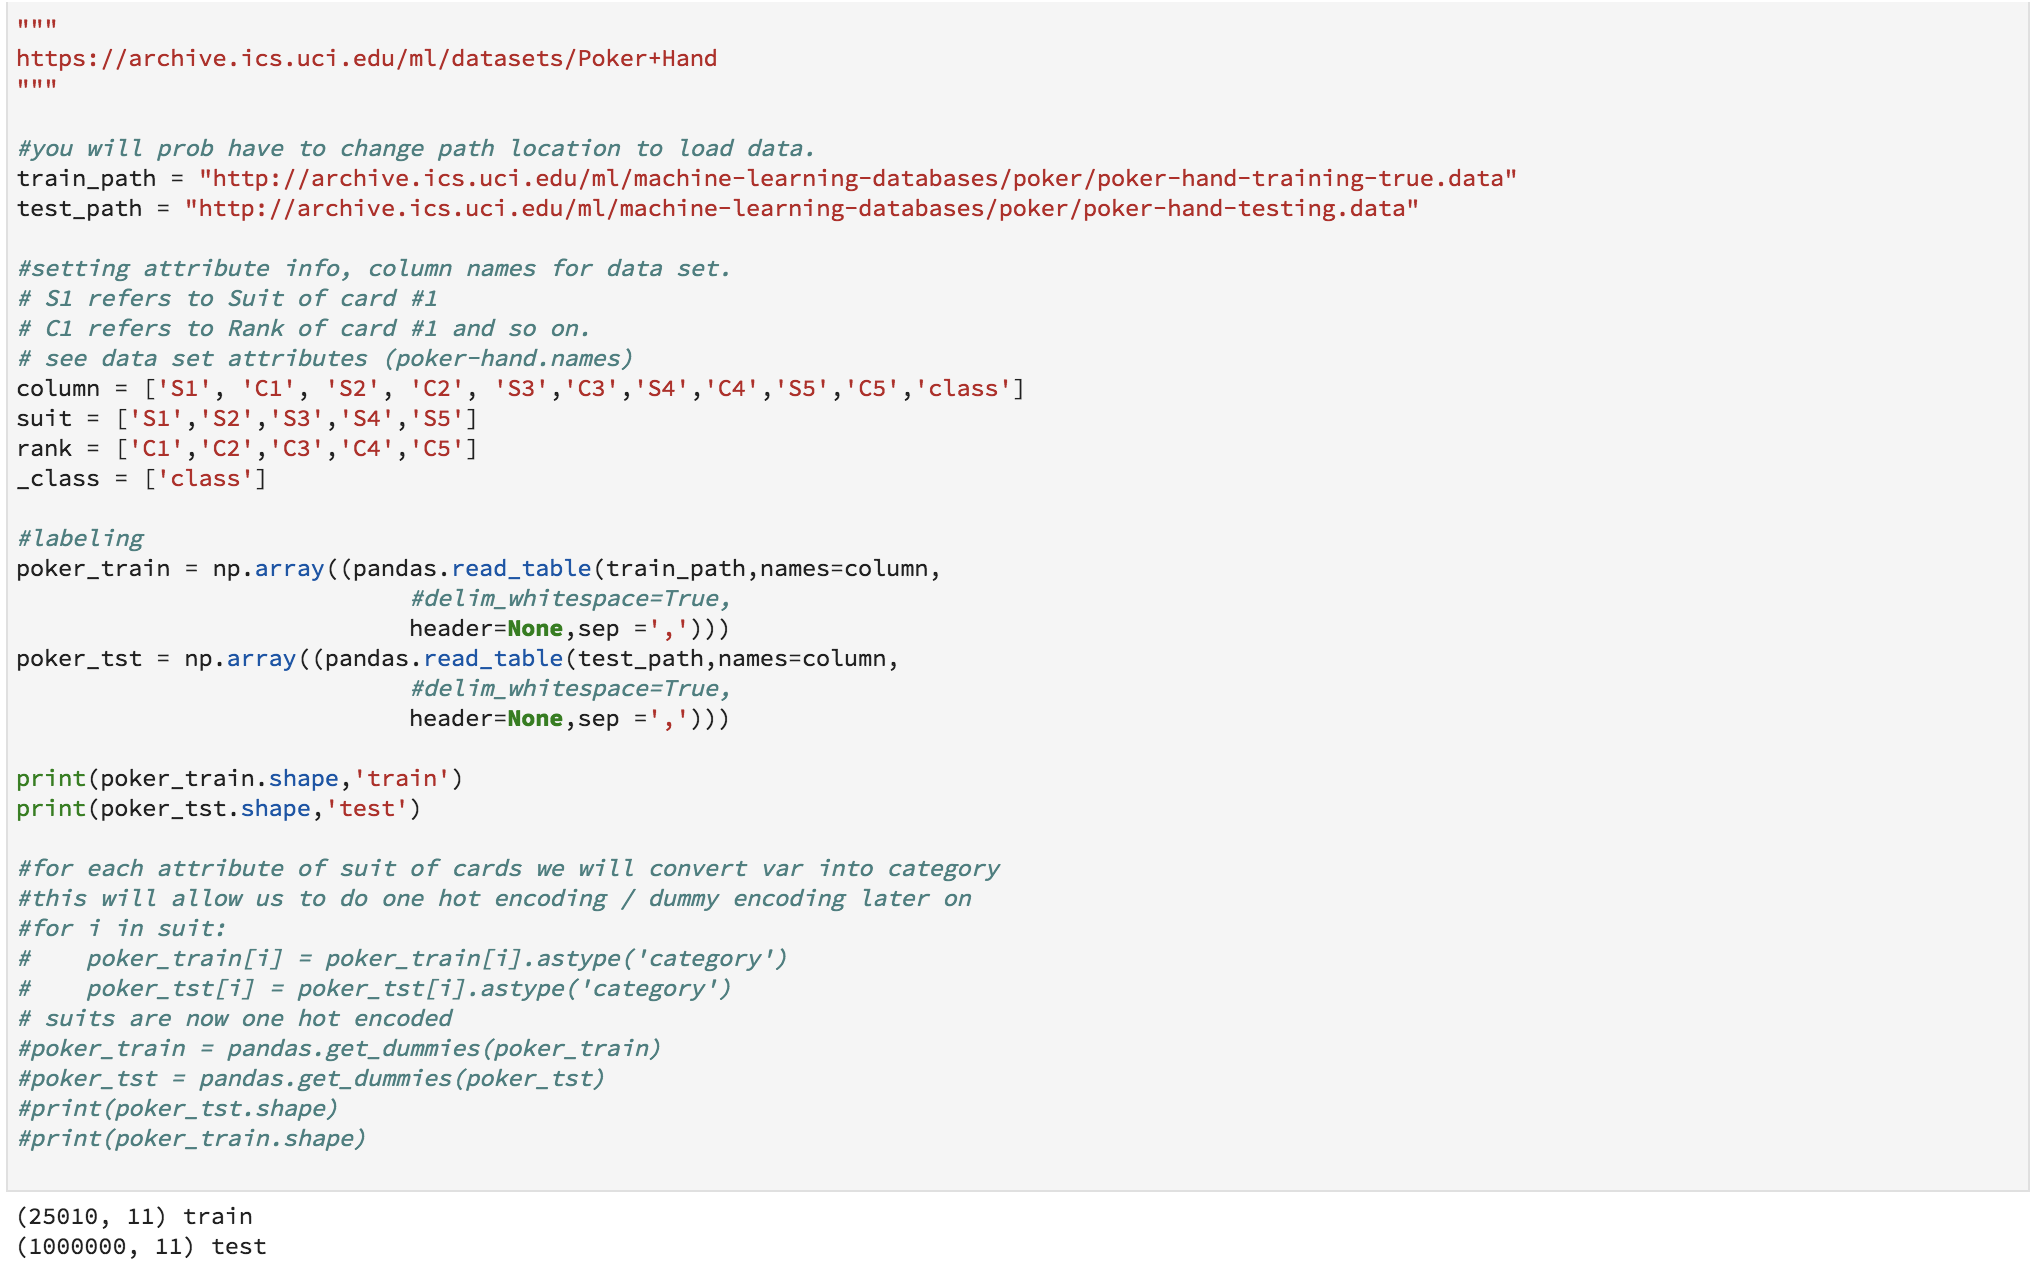
\includegraphics{setup_data_CNN-V2.png}
\caption{}
\end{figure}

    Build the CNN model:

    \begin{figure}[htbp]
\centering
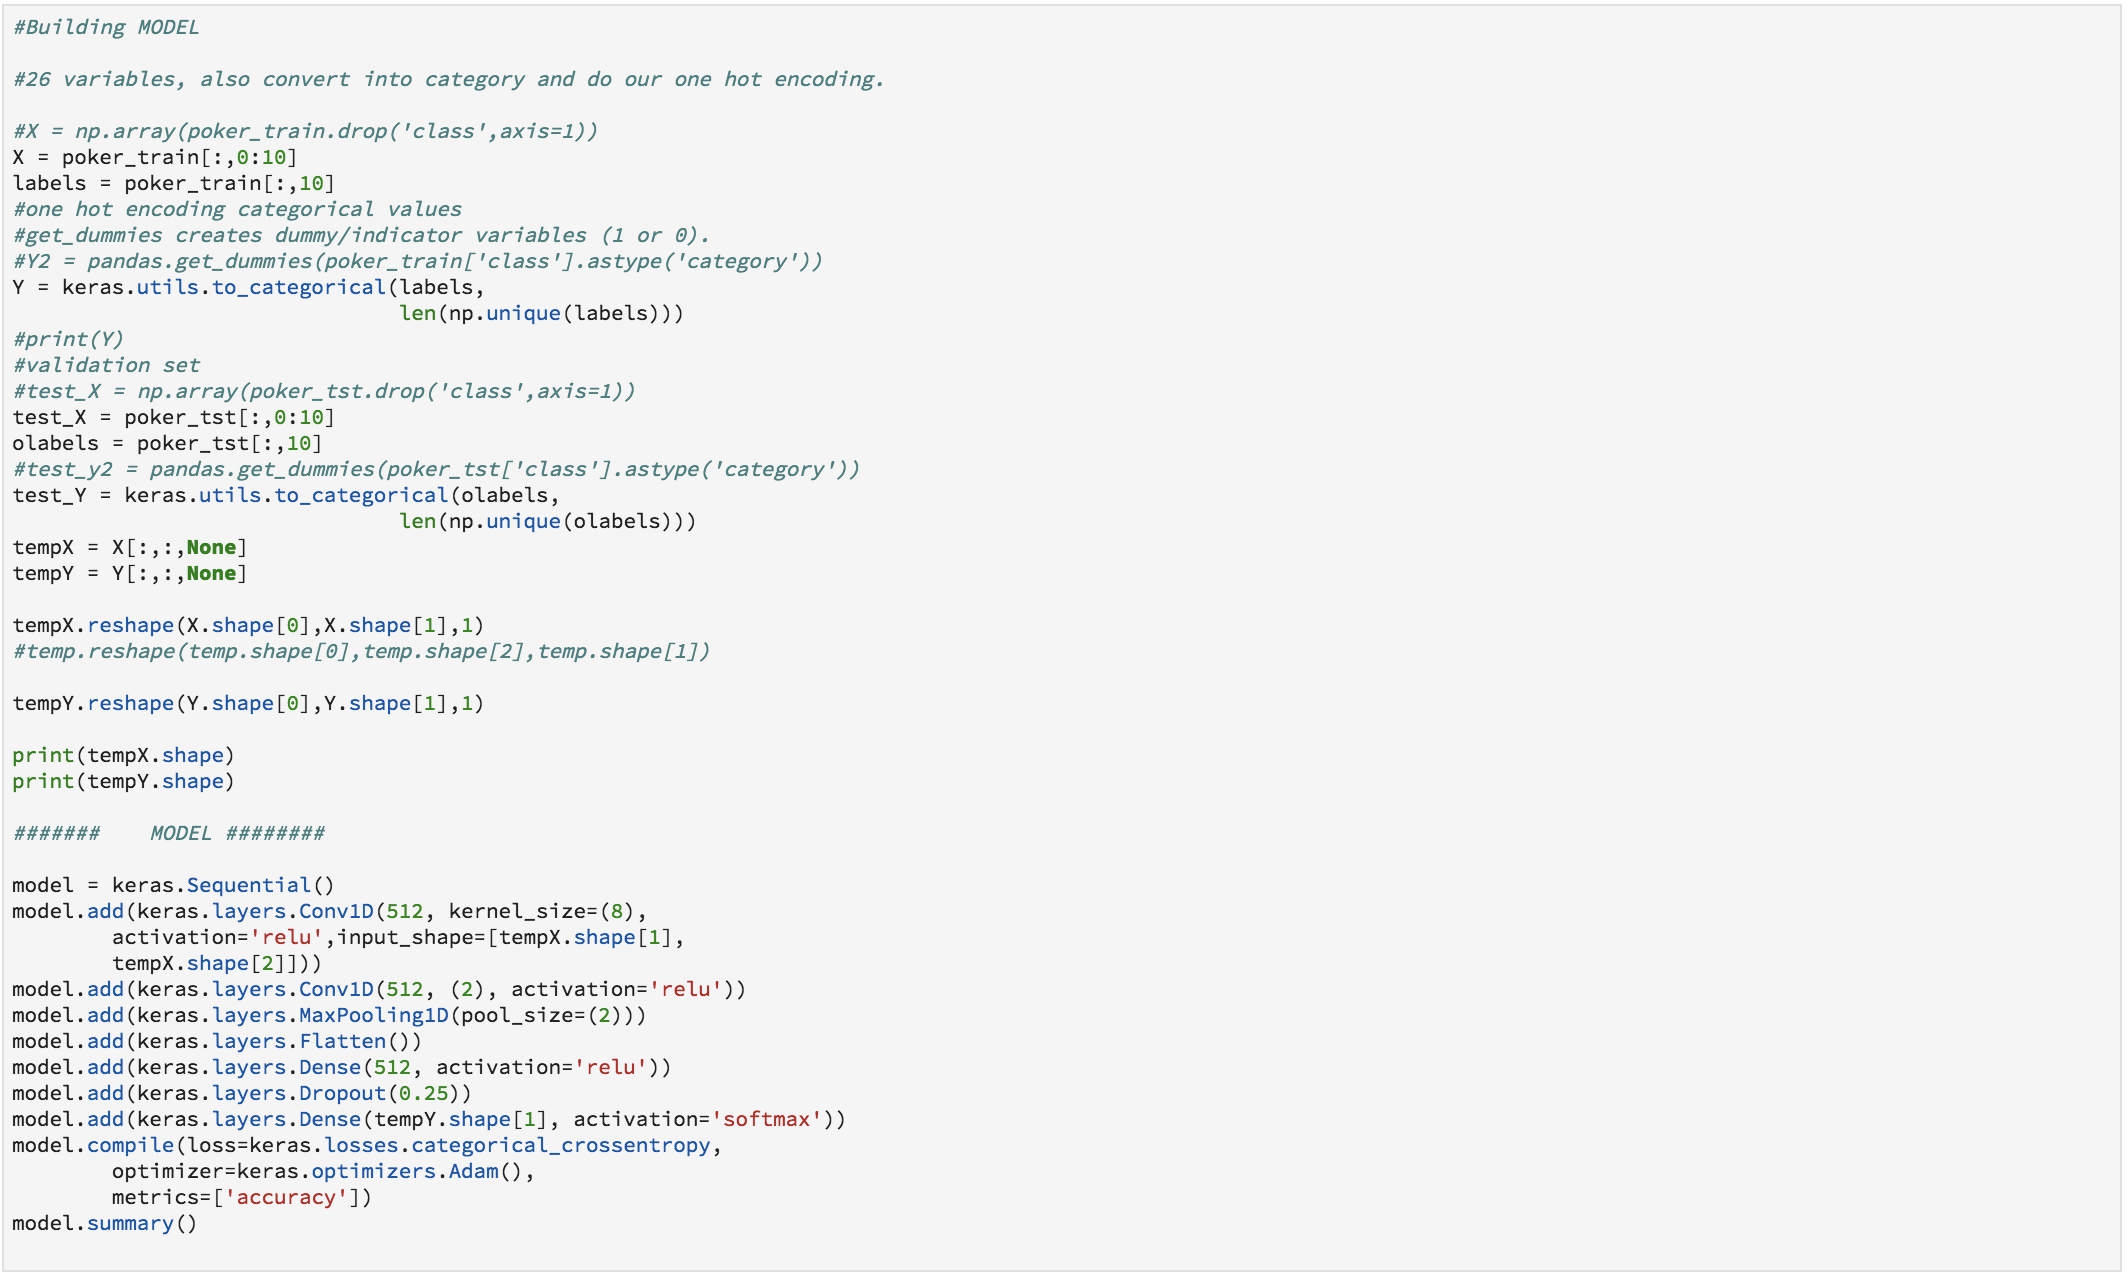
\includegraphics{build_CNN_model-V2.png}
\caption{}
\end{figure}

    \begin{figure}[htbp]
\centering
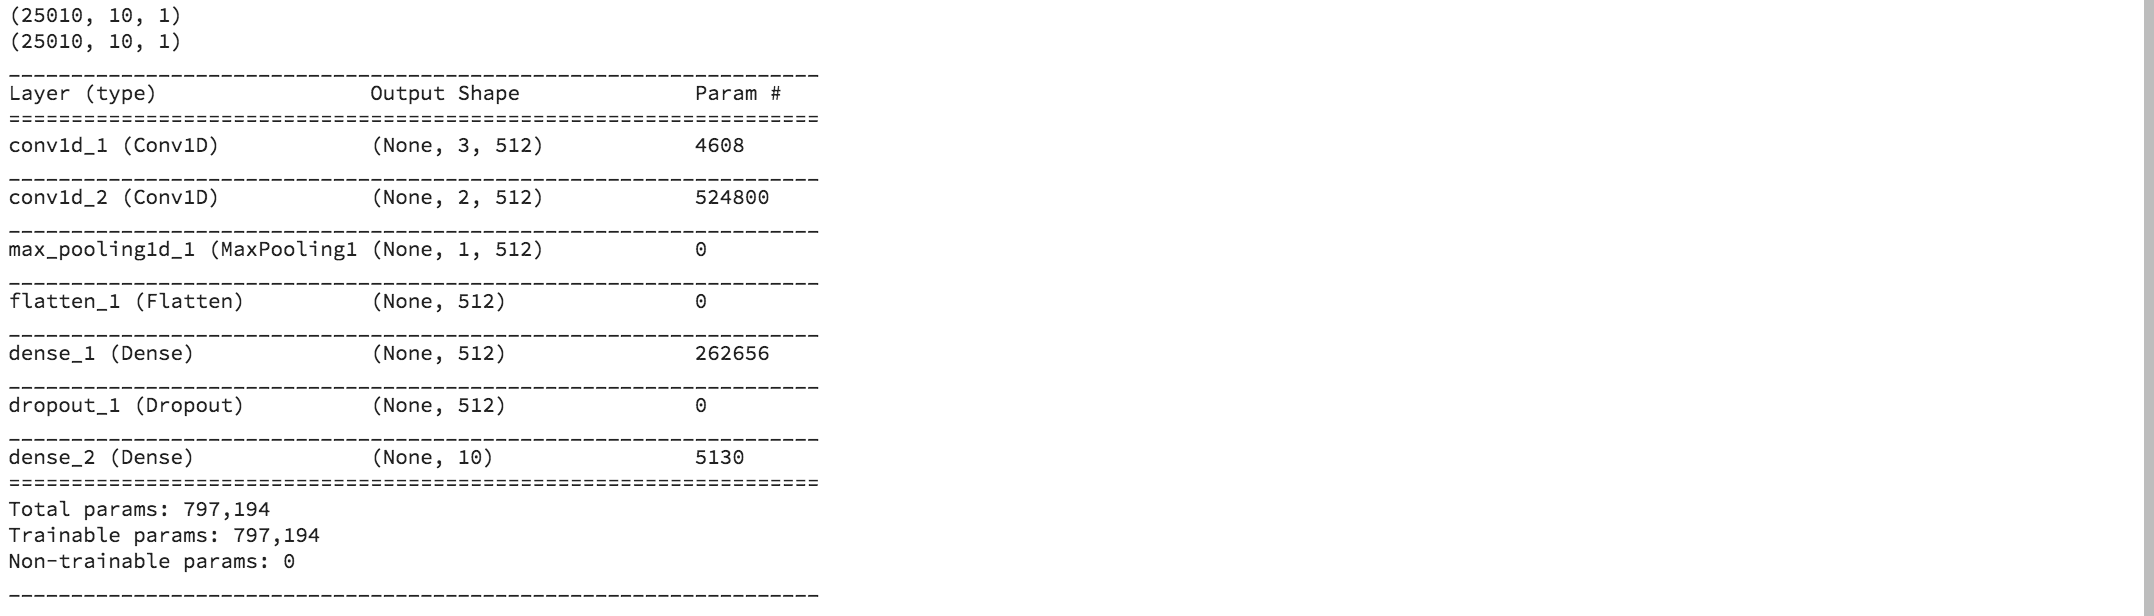
\includegraphics{build_CNN_model-V2-PARA.png}
\caption{}
\end{figure}

    Time to do the training!

    \begin{figure}[htbp]
\centering
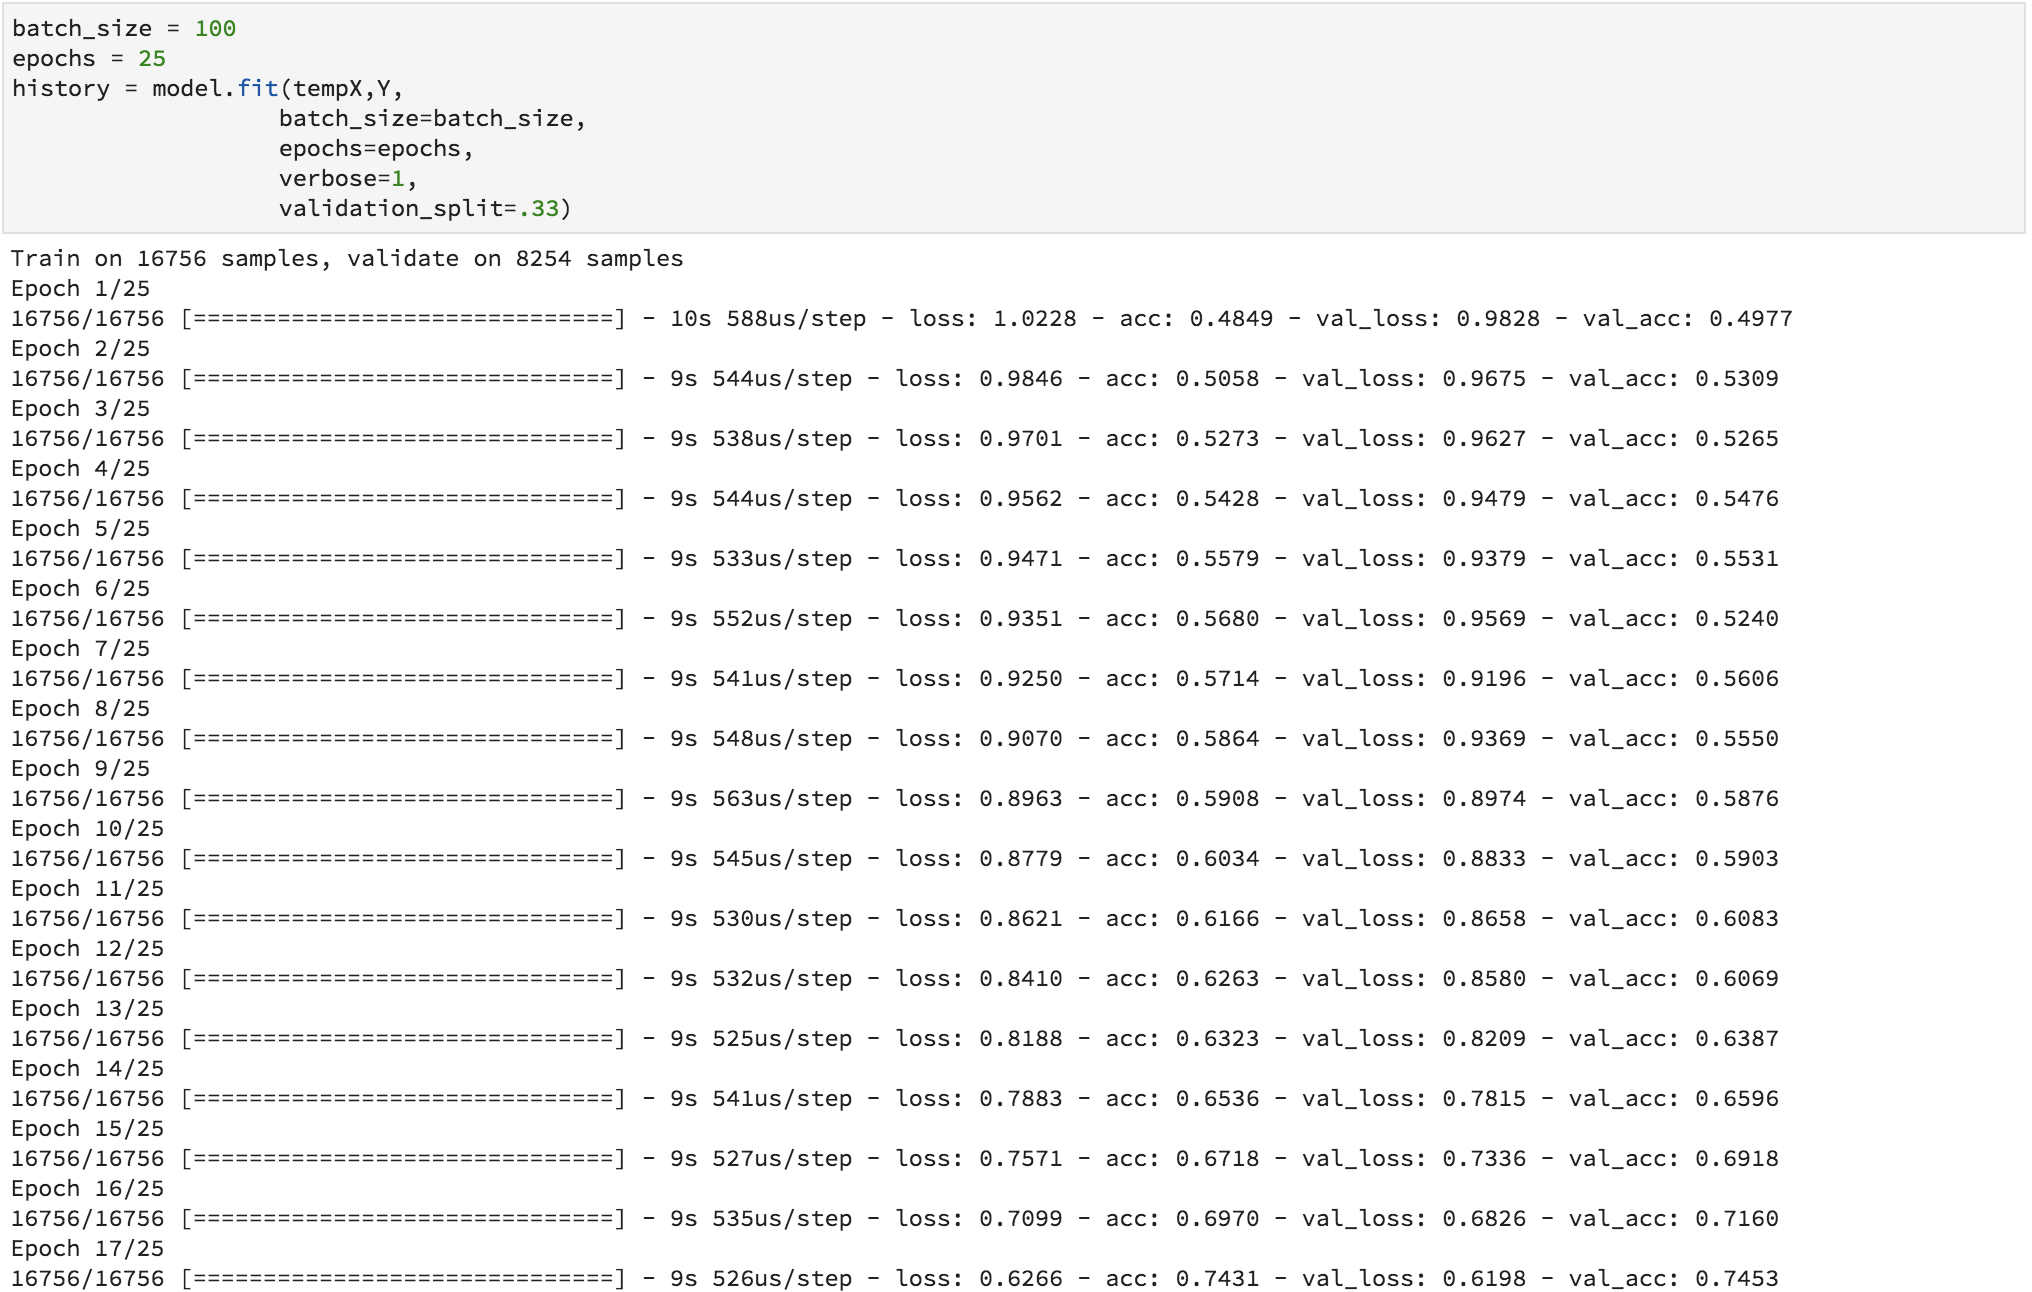
\includegraphics{train_CNN-V2.png}
\caption{}
\end{figure}

    \begin{figure}[htbp]
\centering
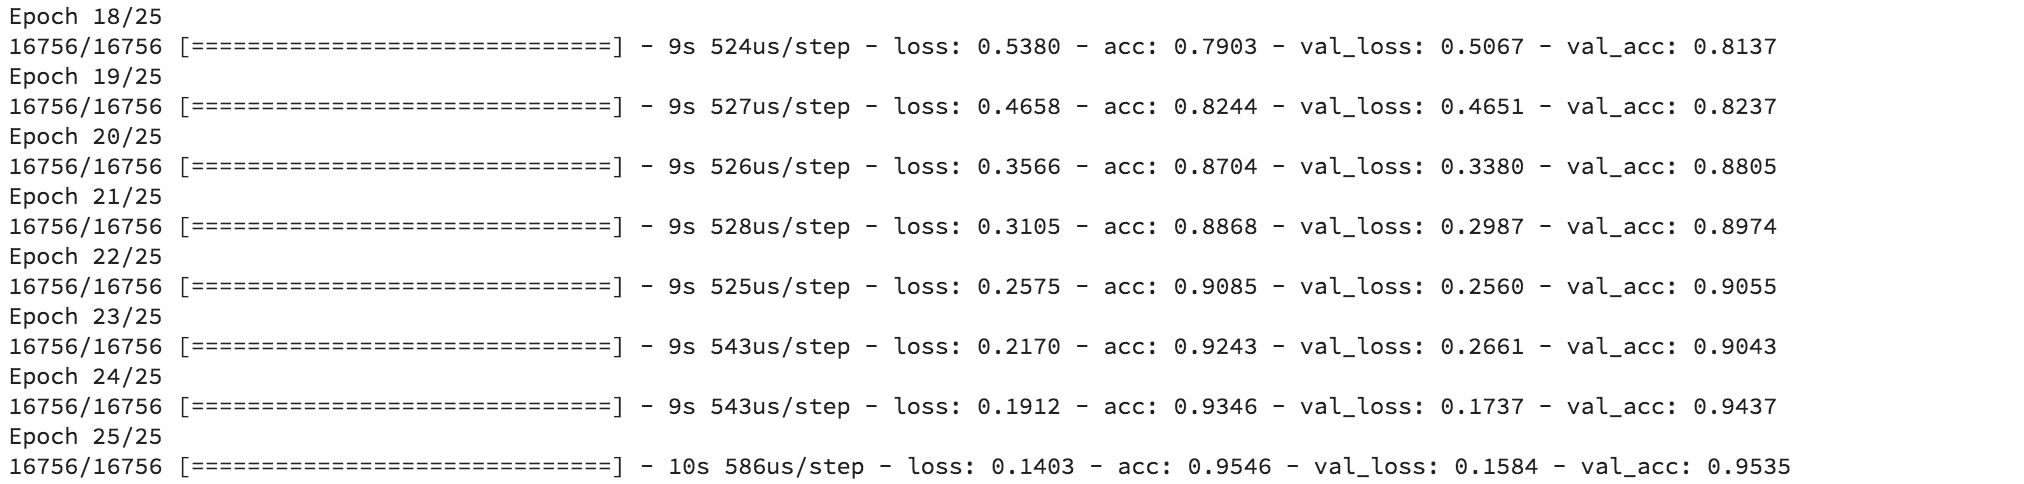
\includegraphics{train_CNN-V2_2.png}
\caption{}
\end{figure}

    Results:

    \begin{figure}[htbp]
\centering
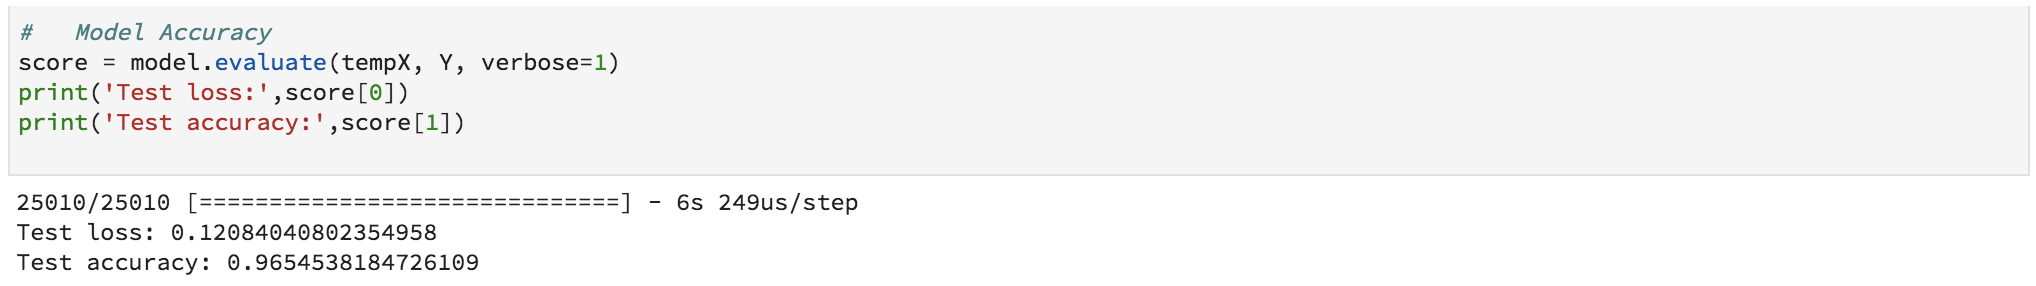
\includegraphics{results_CNN-V2.png}
\caption{}
\end{figure}

    \begin{figure}[htbp]
\centering
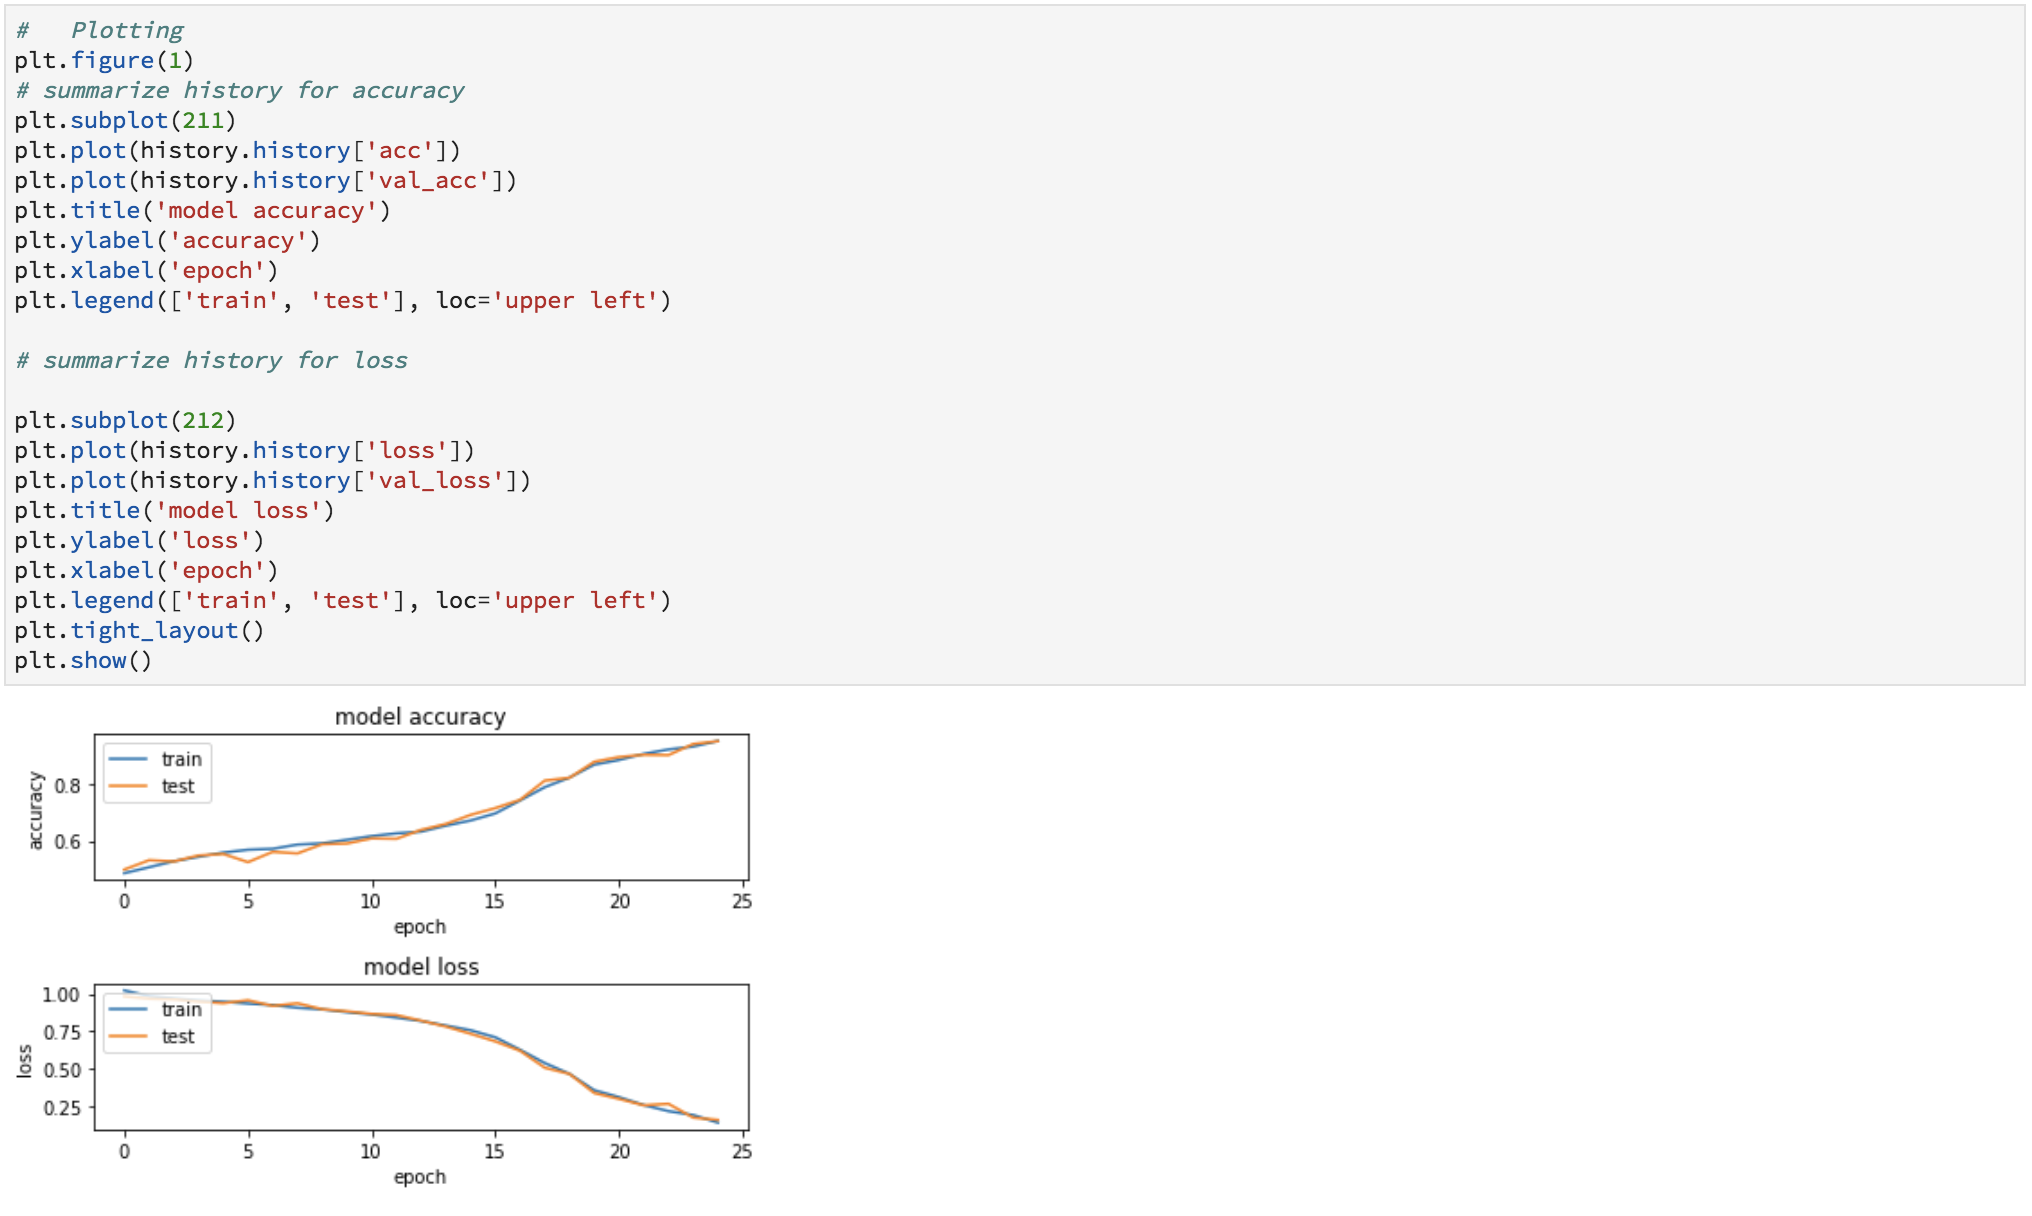
\includegraphics{CNN_graph-V2.png}
\caption{title}
\end{figure}

    As you can see, this performed marginally worse than the Feed-Forward
Neural Network.

    \paragraph{Let's play some poker against the Convolutional Neural
Network!
:}\label{lets-play-some-poker-against-the-convolutional-neural-network}

    Time to take on another AI.

Remember it plays the game in the same way as the Feed-Forward Neural
Network.

    \begin{Verbatim}[commandchars=\\\{\}]
{\color{incolor}In [{\color{incolor}152}]:} \PY{k+kn}{from} \PY{n+nn}{treys} \PY{k}{import} \PY{n}{Deck}\PY{p}{,}\PY{n}{Card}\PY{p}{,}\PY{n}{Evaluator}
          \PY{k+kn}{import} \PY{n+nn}{keras}
          \PY{k+kn}{import} \PY{n+nn}{pandas} \PY{k}{as} \PY{n+nn}{pd}
          \PY{k+kn}{import} \PY{n+nn}{numpy} \PY{k}{as} \PY{n+nn}{np}
          \PY{k+kn}{from} \PY{n+nn}{keras}\PY{n+nn}{.}\PY{n+nn}{models} \PY{k}{import} \PY{n}{load\PYZus{}model}
          
          \PY{n}{deck}\PY{o}{=}\PY{n}{Deck}\PY{p}{(}\PY{p}{)}
          \PY{n}{evaluator}\PY{o}{=}\PY{n}{Evaluator}\PY{p}{(}\PY{p}{)}
          \PY{n}{trans} \PY{o}{=} \PY{p}{\PYZob{}}\PY{l+s+s1}{\PYZsq{}}\PY{l+s+s1}{Ah}\PY{l+s+s1}{\PYZsq{}}\PY{p}{:} \PY{p}{[}\PY{l+m+mi}{1}\PY{p}{,}\PY{l+m+mi}{1}\PY{p}{]}\PY{p}{,} \PY{l+s+s1}{\PYZsq{}}\PY{l+s+s1}{2h}\PY{l+s+s1}{\PYZsq{}}\PY{p}{:} \PY{p}{[}\PY{l+m+mi}{1}\PY{p}{,}\PY{l+m+mi}{2}\PY{p}{]}\PY{p}{,} \PY{l+s+s1}{\PYZsq{}}\PY{l+s+s1}{3h}\PY{l+s+s1}{\PYZsq{}}\PY{p}{:} \PY{p}{[}\PY{l+m+mi}{1}\PY{p}{,}\PY{l+m+mi}{3}\PY{p}{]}\PY{p}{,} \PY{l+s+s1}{\PYZsq{}}\PY{l+s+s1}{4h}\PY{l+s+s1}{\PYZsq{}}\PY{p}{:} \PY{p}{[}\PY{l+m+mi}{1}\PY{p}{,}\PY{l+m+mi}{4}\PY{p}{]}\PY{p}{,}\PY{l+s+s1}{\PYZsq{}}\PY{l+s+s1}{5h}\PY{l+s+s1}{\PYZsq{}}\PY{p}{:} \PY{p}{[}\PY{l+m+mi}{1}\PY{p}{,}\PY{l+m+mi}{5}\PY{p}{]}\PY{p}{,} \PY{l+s+s1}{\PYZsq{}}\PY{l+s+s1}{6h}\PY{l+s+s1}{\PYZsq{}}\PY{p}{:} \PY{p}{[}\PY{l+m+mi}{1}\PY{p}{,}\PY{l+m+mi}{6}\PY{p}{]}\PY{p}{,} \PY{l+s+s1}{\PYZsq{}}\PY{l+s+s1}{7h}\PY{l+s+s1}{\PYZsq{}}\PY{p}{:} \PY{p}{[}\PY{l+m+mi}{1}\PY{p}{,}\PY{l+m+mi}{7}\PY{p}{]}\PY{p}{,} \PY{l+s+s1}{\PYZsq{}}\PY{l+s+s1}{8h}\PY{l+s+s1}{\PYZsq{}}\PY{p}{:} \PY{p}{[}\PY{l+m+mi}{1}\PY{p}{,}\PY{l+m+mi}{8}\PY{p}{]}\PY{p}{,} \PY{l+s+s1}{\PYZsq{}}\PY{l+s+s1}{9h}\PY{l+s+s1}{\PYZsq{}}\PY{p}{:} \PY{p}{[}\PY{l+m+mi}{1}\PY{p}{,}\PY{l+m+mi}{9}\PY{p}{]}\PY{p}{,} \PY{l+s+s1}{\PYZsq{}}\PY{l+s+s1}{Th}\PY{l+s+s1}{\PYZsq{}}\PY{p}{:} \PY{p}{[}\PY{l+m+mi}{1}\PY{p}{,}\PY{l+m+mi}{10}\PY{p}{]}\PY{p}{,}\PY{l+s+s1}{\PYZsq{}}\PY{l+s+s1}{Jh}\PY{l+s+s1}{\PYZsq{}}\PY{p}{:} \PY{p}{[}\PY{l+m+mi}{1}\PY{p}{,}\PY{l+m+mi}{11}\PY{p}{]}\PY{p}{,} \PY{l+s+s1}{\PYZsq{}}\PY{l+s+s1}{Qh}\PY{l+s+s1}{\PYZsq{}}\PY{p}{:} \PY{p}{[}\PY{l+m+mi}{1}\PY{p}{,}\PY{l+m+mi}{12}\PY{p}{]}\PY{p}{,} \PY{l+s+s1}{\PYZsq{}}\PY{l+s+s1}{Kh}\PY{l+s+s1}{\PYZsq{}}\PY{p}{:} \PY{p}{[}\PY{l+m+mi}{1}\PY{p}{,}\PY{l+m+mi}{13}\PY{p}{]}\PY{p}{,}
                  \PY{l+s+s1}{\PYZsq{}}\PY{l+s+s1}{As}\PY{l+s+s1}{\PYZsq{}}\PY{p}{:} \PY{p}{[}\PY{l+m+mi}{2}\PY{p}{,}\PY{l+m+mi}{1}\PY{p}{]}\PY{p}{,} \PY{l+s+s1}{\PYZsq{}}\PY{l+s+s1}{2s}\PY{l+s+s1}{\PYZsq{}}\PY{p}{:} \PY{p}{[}\PY{l+m+mi}{2}\PY{p}{,}\PY{l+m+mi}{2}\PY{p}{]}\PY{p}{,} \PY{l+s+s1}{\PYZsq{}}\PY{l+s+s1}{3s}\PY{l+s+s1}{\PYZsq{}}\PY{p}{:} \PY{p}{[}\PY{l+m+mi}{2}\PY{p}{,}\PY{l+m+mi}{3}\PY{p}{]}\PY{p}{,} \PY{l+s+s1}{\PYZsq{}}\PY{l+s+s1}{4s}\PY{l+s+s1}{\PYZsq{}}\PY{p}{:} \PY{p}{[}\PY{l+m+mi}{2}\PY{p}{,}\PY{l+m+mi}{4}\PY{p}{]}\PY{p}{,}\PY{l+s+s1}{\PYZsq{}}\PY{l+s+s1}{5s}\PY{l+s+s1}{\PYZsq{}}\PY{p}{:} \PY{p}{[}\PY{l+m+mi}{2}\PY{p}{,}\PY{l+m+mi}{5}\PY{p}{]}\PY{p}{,} \PY{l+s+s1}{\PYZsq{}}\PY{l+s+s1}{6s}\PY{l+s+s1}{\PYZsq{}}\PY{p}{:} \PY{p}{[}\PY{l+m+mi}{2}\PY{p}{,}\PY{l+m+mi}{6}\PY{p}{]}\PY{p}{,} \PY{l+s+s1}{\PYZsq{}}\PY{l+s+s1}{7s}\PY{l+s+s1}{\PYZsq{}}\PY{p}{:} \PY{p}{[}\PY{l+m+mi}{2}\PY{p}{,}\PY{l+m+mi}{7}\PY{p}{]}\PY{p}{,} \PY{l+s+s1}{\PYZsq{}}\PY{l+s+s1}{8s}\PY{l+s+s1}{\PYZsq{}}\PY{p}{:} \PY{p}{[}\PY{l+m+mi}{2}\PY{p}{,}\PY{l+m+mi}{8}\PY{p}{]}\PY{p}{,} \PY{l+s+s1}{\PYZsq{}}\PY{l+s+s1}{9s}\PY{l+s+s1}{\PYZsq{}}\PY{p}{:} \PY{p}{[}\PY{l+m+mi}{2}\PY{p}{,}\PY{l+m+mi}{9}\PY{p}{]}\PY{p}{,} \PY{l+s+s1}{\PYZsq{}}\PY{l+s+s1}{Ts}\PY{l+s+s1}{\PYZsq{}}\PY{p}{:} \PY{p}{[}\PY{l+m+mi}{2}\PY{p}{,}\PY{l+m+mi}{10}\PY{p}{]}\PY{p}{,}\PY{l+s+s1}{\PYZsq{}}\PY{l+s+s1}{Js}\PY{l+s+s1}{\PYZsq{}}\PY{p}{:} \PY{p}{[}\PY{l+m+mi}{2}\PY{p}{,}\PY{l+m+mi}{11}\PY{p}{]}\PY{p}{,} \PY{l+s+s1}{\PYZsq{}}\PY{l+s+s1}{Qs}\PY{l+s+s1}{\PYZsq{}}\PY{p}{:} \PY{p}{[}\PY{l+m+mi}{2}\PY{p}{,}\PY{l+m+mi}{12}\PY{p}{]}\PY{p}{,} \PY{l+s+s1}{\PYZsq{}}\PY{l+s+s1}{Ks}\PY{l+s+s1}{\PYZsq{}}\PY{p}{:} \PY{p}{[}\PY{l+m+mi}{2}\PY{p}{,}\PY{l+m+mi}{13}\PY{p}{]}\PY{p}{,}
                  \PY{l+s+s1}{\PYZsq{}}\PY{l+s+s1}{Ad}\PY{l+s+s1}{\PYZsq{}}\PY{p}{:} \PY{p}{[}\PY{l+m+mi}{3}\PY{p}{,}\PY{l+m+mi}{1}\PY{p}{]}\PY{p}{,} \PY{l+s+s1}{\PYZsq{}}\PY{l+s+s1}{2d}\PY{l+s+s1}{\PYZsq{}}\PY{p}{:} \PY{p}{[}\PY{l+m+mi}{3}\PY{p}{,}\PY{l+m+mi}{2}\PY{p}{]}\PY{p}{,} \PY{l+s+s1}{\PYZsq{}}\PY{l+s+s1}{3d}\PY{l+s+s1}{\PYZsq{}}\PY{p}{:} \PY{p}{[}\PY{l+m+mi}{3}\PY{p}{,}\PY{l+m+mi}{3}\PY{p}{]}\PY{p}{,} \PY{l+s+s1}{\PYZsq{}}\PY{l+s+s1}{4d}\PY{l+s+s1}{\PYZsq{}}\PY{p}{:} \PY{p}{[}\PY{l+m+mi}{3}\PY{p}{,}\PY{l+m+mi}{4}\PY{p}{]}\PY{p}{,}\PY{l+s+s1}{\PYZsq{}}\PY{l+s+s1}{5d}\PY{l+s+s1}{\PYZsq{}}\PY{p}{:} \PY{p}{[}\PY{l+m+mi}{3}\PY{p}{,}\PY{l+m+mi}{5}\PY{p}{]}\PY{p}{,} \PY{l+s+s1}{\PYZsq{}}\PY{l+s+s1}{6d}\PY{l+s+s1}{\PYZsq{}}\PY{p}{:} \PY{p}{[}\PY{l+m+mi}{3}\PY{p}{,}\PY{l+m+mi}{6}\PY{p}{]}\PY{p}{,} \PY{l+s+s1}{\PYZsq{}}\PY{l+s+s1}{7d}\PY{l+s+s1}{\PYZsq{}}\PY{p}{:} \PY{p}{[}\PY{l+m+mi}{3}\PY{p}{,}\PY{l+m+mi}{7}\PY{p}{]}\PY{p}{,} \PY{l+s+s1}{\PYZsq{}}\PY{l+s+s1}{8d}\PY{l+s+s1}{\PYZsq{}}\PY{p}{:} \PY{p}{[}\PY{l+m+mi}{3}\PY{p}{,}\PY{l+m+mi}{8}\PY{p}{]}\PY{p}{,} \PY{l+s+s1}{\PYZsq{}}\PY{l+s+s1}{9d}\PY{l+s+s1}{\PYZsq{}}\PY{p}{:} \PY{p}{[}\PY{l+m+mi}{3}\PY{p}{,}\PY{l+m+mi}{9}\PY{p}{]}\PY{p}{,} \PY{l+s+s1}{\PYZsq{}}\PY{l+s+s1}{Td}\PY{l+s+s1}{\PYZsq{}}\PY{p}{:} \PY{p}{[}\PY{l+m+mi}{3}\PY{p}{,}\PY{l+m+mi}{10}\PY{p}{]}\PY{p}{,}\PY{l+s+s1}{\PYZsq{}}\PY{l+s+s1}{Jd}\PY{l+s+s1}{\PYZsq{}}\PY{p}{:} \PY{p}{[}\PY{l+m+mi}{3}\PY{p}{,}\PY{l+m+mi}{11}\PY{p}{]}\PY{p}{,} \PY{l+s+s1}{\PYZsq{}}\PY{l+s+s1}{Qd}\PY{l+s+s1}{\PYZsq{}}\PY{p}{:} \PY{p}{[}\PY{l+m+mi}{3}\PY{p}{,}\PY{l+m+mi}{12}\PY{p}{]}\PY{p}{,} \PY{l+s+s1}{\PYZsq{}}\PY{l+s+s1}{Kd}\PY{l+s+s1}{\PYZsq{}}\PY{p}{:} \PY{p}{[}\PY{l+m+mi}{3}\PY{p}{,}\PY{l+m+mi}{13}\PY{p}{]}\PY{p}{,}
                  \PY{l+s+s1}{\PYZsq{}}\PY{l+s+s1}{Ac}\PY{l+s+s1}{\PYZsq{}}\PY{p}{:} \PY{p}{[}\PY{l+m+mi}{4}\PY{p}{,}\PY{l+m+mi}{1}\PY{p}{]}\PY{p}{,} \PY{l+s+s1}{\PYZsq{}}\PY{l+s+s1}{2c}\PY{l+s+s1}{\PYZsq{}}\PY{p}{:} \PY{p}{[}\PY{l+m+mi}{4}\PY{p}{,}\PY{l+m+mi}{2}\PY{p}{]}\PY{p}{,} \PY{l+s+s1}{\PYZsq{}}\PY{l+s+s1}{3c}\PY{l+s+s1}{\PYZsq{}}\PY{p}{:} \PY{p}{[}\PY{l+m+mi}{4}\PY{p}{,}\PY{l+m+mi}{3}\PY{p}{]}\PY{p}{,} \PY{l+s+s1}{\PYZsq{}}\PY{l+s+s1}{4c}\PY{l+s+s1}{\PYZsq{}}\PY{p}{:} \PY{p}{[}\PY{l+m+mi}{4}\PY{p}{,}\PY{l+m+mi}{4}\PY{p}{]}\PY{p}{,}\PY{l+s+s1}{\PYZsq{}}\PY{l+s+s1}{5c}\PY{l+s+s1}{\PYZsq{}}\PY{p}{:} \PY{p}{[}\PY{l+m+mi}{4}\PY{p}{,}\PY{l+m+mi}{5}\PY{p}{]}\PY{p}{,} \PY{l+s+s1}{\PYZsq{}}\PY{l+s+s1}{6c}\PY{l+s+s1}{\PYZsq{}}\PY{p}{:} \PY{p}{[}\PY{l+m+mi}{4}\PY{p}{,}\PY{l+m+mi}{6}\PY{p}{]}\PY{p}{,} \PY{l+s+s1}{\PYZsq{}}\PY{l+s+s1}{7c}\PY{l+s+s1}{\PYZsq{}}\PY{p}{:} \PY{p}{[}\PY{l+m+mi}{4}\PY{p}{,}\PY{l+m+mi}{7}\PY{p}{]}\PY{p}{,} \PY{l+s+s1}{\PYZsq{}}\PY{l+s+s1}{8c}\PY{l+s+s1}{\PYZsq{}}\PY{p}{:} \PY{p}{[}\PY{l+m+mi}{4}\PY{p}{,}\PY{l+m+mi}{8}\PY{p}{]}\PY{p}{,} \PY{l+s+s1}{\PYZsq{}}\PY{l+s+s1}{9c}\PY{l+s+s1}{\PYZsq{}}\PY{p}{:} \PY{p}{[}\PY{l+m+mi}{4}\PY{p}{,}\PY{l+m+mi}{9}\PY{p}{]}\PY{p}{,} \PY{l+s+s1}{\PYZsq{}}\PY{l+s+s1}{Tc}\PY{l+s+s1}{\PYZsq{}}\PY{p}{:} \PY{p}{[}\PY{l+m+mi}{4}\PY{p}{,}\PY{l+m+mi}{10}\PY{p}{]}\PY{p}{,}\PY{l+s+s1}{\PYZsq{}}\PY{l+s+s1}{Jc}\PY{l+s+s1}{\PYZsq{}}\PY{p}{:} \PY{p}{[}\PY{l+m+mi}{4}\PY{p}{,}\PY{l+m+mi}{11}\PY{p}{]}\PY{p}{,} \PY{l+s+s1}{\PYZsq{}}\PY{l+s+s1}{Qc}\PY{l+s+s1}{\PYZsq{}}\PY{p}{:} \PY{p}{[}\PY{l+m+mi}{4}\PY{p}{,}\PY{l+m+mi}{12}\PY{p}{]}\PY{p}{,} \PY{l+s+s1}{\PYZsq{}}\PY{l+s+s1}{Kc}\PY{l+s+s1}{\PYZsq{}}\PY{p}{:} \PY{p}{[}\PY{l+m+mi}{4}\PY{p}{,}\PY{l+m+mi}{13}\PY{p}{]}
                  \PY{p}{\PYZcb{}} \PY{c+c1}{\PYZsh{}dict creation}
\end{Verbatim}


    \begin{Verbatim}[commandchars=\\\{\}]
{\color{incolor}In [{\color{incolor}153}]:} \PY{n}{player1\PYZus{}hand}\PY{o}{=}\PY{n}{deck}\PY{o}{.}\PY{n}{draw}\PY{p}{(}\PY{l+m+mi}{5}\PY{p}{)} \PY{c+c1}{\PYZsh{}draw initial hands}
          \PY{n}{nn\PYZus{}hand}\PY{o}{=}\PY{n}{deck}\PY{o}{.}\PY{n}{draw}\PY{p}{(}\PY{l+m+mi}{5}\PY{p}{)}
          
          \PY{n+nb}{print} \PY{p}{(}\PY{l+s+s2}{\PYZdq{}}\PY{l+s+s2}{Your hand: }\PY{l+s+s2}{\PYZdq{}}\PY{p}{)}\PY{c+c1}{\PYZsh{} prints initial hands}
          \PY{n}{Card}\PY{o}{.}\PY{n}{print\PYZus{}pretty\PYZus{}cards}\PY{p}{(}\PY{n}{player1\PYZus{}hand}\PY{p}{)}
\end{Verbatim}


    \begin{Verbatim}[commandchars=\\\{\}]
Your hand: 
 [J♣],[3\textcolor{ansi-red}{♥}],[5♠],[T♣],[J\textcolor{ansi-red}{♥}] 

    \end{Verbatim}

    Please specify which cards you would like to discard.

Your cards are ordered 0-4 from left to right.

    \begin{Verbatim}[commandchars=\\\{\}]
{\color{incolor}In [{\color{incolor}154}]:} \PY{n}{new\PYZus{}hand}\PY{o}{=}\PY{p}{[}\PY{l+m+mi}{0}\PY{p}{,}\PY{l+m+mi}{0}\PY{p}{,}\PY{l+m+mi}{0}\PY{p}{,}\PY{l+m+mi}{0}\PY{p}{,}\PY{l+m+mi}{0}\PY{p}{]}
          \PY{n+nb}{print}\PY{p}{(}\PY{l+s+s1}{\PYZsq{}}\PY{l+s+s1}{Please enter yes or no to indicate your choice:}\PY{l+s+s1}{\PYZsq{}}\PY{p}{)}
          \PY{n+nb}{print}\PY{p}{(}\PY{l+s+s1}{\PYZsq{}}\PY{l+s+s1}{Would you like to discard your card at position 0?}\PY{l+s+s1}{\PYZsq{}}\PY{p}{,}\PY{l+s+s1}{\PYZsq{}}\PY{l+s+se}{\PYZbs{}n}\PY{l+s+s1}{\PYZsq{}}\PY{p}{)}
          \PY{n}{zero}\PY{o}{=}\PY{n+nb}{input}\PY{p}{(}\PY{p}{)}
          \PY{n+nb}{print}\PY{p}{(}\PY{l+s+s1}{\PYZsq{}}\PY{l+s+s1}{Would you like to discard your card at position 1?}\PY{l+s+s1}{\PYZsq{}}\PY{p}{,}\PY{l+s+s1}{\PYZsq{}}\PY{l+s+se}{\PYZbs{}n}\PY{l+s+s1}{\PYZsq{}}\PY{p}{)}
          \PY{n}{one}\PY{o}{=}\PY{n+nb}{input}\PY{p}{(}\PY{p}{)}
          \PY{n+nb}{print}\PY{p}{(}\PY{l+s+s1}{\PYZsq{}}\PY{l+s+s1}{Would you like to discard your card at position 2?}\PY{l+s+s1}{\PYZsq{}}\PY{p}{,}\PY{l+s+s1}{\PYZsq{}}\PY{l+s+se}{\PYZbs{}n}\PY{l+s+s1}{\PYZsq{}}\PY{p}{)}
          \PY{n}{two}\PY{o}{=}\PY{n+nb}{input}\PY{p}{(}\PY{p}{)}
          \PY{n+nb}{print}\PY{p}{(}\PY{l+s+s1}{\PYZsq{}}\PY{l+s+s1}{Would you like to discard your card at position 3?}\PY{l+s+s1}{\PYZsq{}}\PY{p}{,}\PY{l+s+s1}{\PYZsq{}}\PY{l+s+se}{\PYZbs{}n}\PY{l+s+s1}{\PYZsq{}}\PY{p}{)}
          \PY{n}{three}\PY{o}{=}\PY{n+nb}{input}\PY{p}{(}\PY{p}{)}
          \PY{n+nb}{print}\PY{p}{(}\PY{l+s+s1}{\PYZsq{}}\PY{l+s+s1}{Would you like to discard your card at position 4?}\PY{l+s+s1}{\PYZsq{}}\PY{p}{,}\PY{l+s+s1}{\PYZsq{}}\PY{l+s+se}{\PYZbs{}n}\PY{l+s+s1}{\PYZsq{}}\PY{p}{)}
          \PY{n}{four}\PY{o}{=}\PY{n+nb}{input}\PY{p}{(}\PY{p}{)}
          \PY{k}{if}\PY{p}{(}\PY{n}{zero}\PY{o}{.}\PY{n}{lower}\PY{p}{(}\PY{p}{)}\PY{o}{==}\PY{l+s+s1}{\PYZsq{}}\PY{l+s+s1}{yes}\PY{l+s+s1}{\PYZsq{}}\PY{p}{)}\PY{p}{:}
              \PY{n}{new\PYZus{}hand}\PY{p}{[}\PY{l+m+mi}{0}\PY{p}{]}\PY{o}{=}\PY{n}{deck}\PY{o}{.}\PY{n}{draw}\PY{p}{(}\PY{l+m+mi}{1}\PY{p}{)}
          \PY{k}{if}\PY{p}{(}\PY{n}{one}\PY{o}{.}\PY{n}{lower}\PY{p}{(}\PY{p}{)}\PY{o}{==}\PY{l+s+s1}{\PYZsq{}}\PY{l+s+s1}{yes}\PY{l+s+s1}{\PYZsq{}}\PY{p}{)}\PY{p}{:}
              \PY{n}{new\PYZus{}hand}\PY{p}{[}\PY{l+m+mi}{1}\PY{p}{]}\PY{o}{=}\PY{n}{deck}\PY{o}{.}\PY{n}{draw}\PY{p}{(}\PY{l+m+mi}{1}\PY{p}{)}
          \PY{k}{if}\PY{p}{(}\PY{n}{two}\PY{o}{.}\PY{n}{lower}\PY{p}{(}\PY{p}{)}\PY{o}{==}\PY{l+s+s1}{\PYZsq{}}\PY{l+s+s1}{yes}\PY{l+s+s1}{\PYZsq{}}\PY{p}{)}\PY{p}{:}
              \PY{n}{new\PYZus{}hand}\PY{p}{[}\PY{l+m+mi}{2}\PY{p}{]}\PY{o}{=}\PY{n}{deck}\PY{o}{.}\PY{n}{draw}\PY{p}{(}\PY{l+m+mi}{1}\PY{p}{)}
          \PY{k}{if}\PY{p}{(}\PY{n}{three}\PY{o}{.}\PY{n}{lower}\PY{p}{(}\PY{p}{)}\PY{o}{==}\PY{l+s+s1}{\PYZsq{}}\PY{l+s+s1}{yes}\PY{l+s+s1}{\PYZsq{}}\PY{p}{)}\PY{p}{:}
              \PY{n}{new\PYZus{}hand}\PY{p}{[}\PY{l+m+mi}{3}\PY{p}{]}\PY{o}{=}\PY{n}{deck}\PY{o}{.}\PY{n}{draw}\PY{p}{(}\PY{l+m+mi}{1}\PY{p}{)}
          \PY{k}{if}\PY{p}{(}\PY{n}{four}\PY{o}{.}\PY{n}{lower}\PY{p}{(}\PY{p}{)}\PY{o}{==}\PY{l+s+s1}{\PYZsq{}}\PY{l+s+s1}{yes}\PY{l+s+s1}{\PYZsq{}}\PY{p}{)}\PY{p}{:}
              \PY{n}{new\PYZus{}hand}\PY{p}{[}\PY{l+m+mi}{4}\PY{p}{]}\PY{o}{=}\PY{n}{deck}\PY{o}{.}\PY{n}{draw}\PY{p}{(}\PY{l+m+mi}{1}\PY{p}{)}
          
          \PY{k}{for} \PY{n}{i} \PY{o+ow}{in} \PY{n+nb}{range}\PY{p}{(}\PY{l+m+mi}{0}\PY{p}{,}\PY{l+m+mi}{5}\PY{p}{)}\PY{p}{:}
              \PY{k}{if}\PY{p}{(}\PY{n}{new\PYZus{}hand}\PY{p}{[}\PY{n}{i}\PY{p}{]}\PY{o}{!=}\PY{l+m+mi}{0}\PY{p}{)}\PY{p}{:}
                  \PY{n}{player1\PYZus{}hand}\PY{p}{[}\PY{n}{i}\PY{p}{]}\PY{o}{=}\PY{n}{new\PYZus{}hand}\PY{p}{[}\PY{n}{i}\PY{p}{]}        
          
          \PY{n+nb}{print}\PY{p}{(}\PY{l+s+s2}{\PYZdq{}}\PY{l+s+s2}{Your current hand is:}\PY{l+s+s2}{\PYZdq{}} \PY{p}{,}\PY{l+s+s1}{\PYZsq{}}\PY{l+s+se}{\PYZbs{}n}\PY{l+s+s1}{\PYZsq{}}\PY{p}{)}
          \PY{n}{Card}\PY{o}{.}\PY{n}{print\PYZus{}pretty\PYZus{}cards}\PY{p}{(}\PY{n}{player1\PYZus{}hand}\PY{p}{)}
\end{Verbatim}


    \begin{Verbatim}[commandchars=\\\{\}]
Please enter yes or no to indicate your choice:
Would you like to discard your card at position 0? 

Would you like to discard your card at position 1? 

Would you like to discard your card at position 2? 

Would you like to discard your card at position 3? 

Would you like to discard your card at position 4? 

Your current hand is: 

 [2\textcolor{ansi-red}{♥}],[3♣],[6♣],[T♠],[K♣] 

    \end{Verbatim}

    \paragraph{Note: You might want to wait \textasciitilde{}20 seconds for
the code in this next cell to
finish...}\label{note-you-might-want-to-wait-20-seconds-for-the-code-in-this-next-cell-to-finish...}

    \begin{Verbatim}[commandchars=\\\{\}]
{\color{incolor}In [{\color{incolor}155}]:} \PY{c+c1}{\PYZsh{}determine what the CNN thinks of the hand}
          \PY{n}{hand\PYZus{}for\PYZus{}nn2}\PY{o}{=}\PY{p}{[}\PY{p}{]}
          \PY{k}{for} \PY{n}{i} \PY{o+ow}{in} \PY{n+nb}{range}\PY{p}{(}\PY{l+m+mi}{0}\PY{p}{,}\PY{l+m+mi}{5}\PY{p}{)}\PY{p}{:}
              \PY{n}{hand\PYZus{}for\PYZus{}nn2}\PY{o}{=}\PY{p}{(}\PY{n}{hand\PYZus{}for\PYZus{}nn2}\PY{o}{+}\PY{n}{trans}\PY{p}{[}\PY{n}{Card}\PY{o}{.}\PY{n}{int\PYZus{}to\PYZus{}str}\PY{p}{(}\PY{n}{nn\PYZus{}hand}\PY{p}{[}\PY{n}{i}\PY{p}{]}\PY{p}{)}\PY{p}{]}\PY{p}{)}
          
              
              
          \PY{n}{model2} \PY{o}{=} \PY{n}{load\PYZus{}model}\PY{p}{(}\PY{l+s+s1}{\PYZsq{}}\PY{l+s+s1}{demo/cnn.h5}\PY{l+s+s1}{\PYZsq{}}\PY{p}{)} \PY{c+c1}{\PYZsh{}ffbnn.h5 is feed forward NN}
          
          \PY{n}{handarray2} \PY{o}{=} \PY{n}{np}\PY{o}{.}\PY{n}{array}\PY{p}{(}\PY{p}{[}\PY{n}{hand\PYZus{}for\PYZus{}nn2}\PY{p}{]}\PY{p}{)} \PY{c+c1}{\PYZsh{}convert hand to np array for input}
              
              
          \PY{n}{handarray2\PYZus{}t} \PY{o}{=} \PY{n}{handarray2}\PY{p}{[}\PY{p}{:}\PY{p}{,}\PY{p}{:}\PY{p}{,}\PY{k+kc}{None}\PY{p}{]}
              
          \PY{n}{handarray2\PYZus{}t}\PY{o}{.}\PY{n}{reshape}\PY{p}{(}\PY{n}{handarray2}\PY{o}{.}\PY{n}{shape}\PY{p}{[}\PY{l+m+mi}{0}\PY{p}{]}\PY{p}{,}\PY{n}{handarray2}\PY{o}{.}\PY{n}{shape}\PY{p}{[}\PY{l+m+mi}{1}\PY{p}{]}\PY{p}{,}\PY{l+m+mi}{1}\PY{p}{)}
             
          \PY{n}{preds2} \PY{o}{=} \PY{n}{model2}\PY{o}{.}\PY{n}{predict}\PY{p}{(}\PY{n}{handarray2\PYZus{}t}\PY{p}{)} \PY{c+c1}{\PYZsh{}calculates probabilities of each class from NN}
          
          \PY{n}{label}\PY{o}{=}\PY{n}{np}\PY{o}{.}\PY{n}{argmax}\PY{p}{(}\PY{n}{preds2}\PY{p}{)}
          
          \PY{c+c1}{\PYZsh{}if nothing in hand}
          \PY{k}{if} \PY{p}{(}\PY{n}{label}\PY{o}{==}\PY{l+m+mi}{0}\PY{p}{)}\PY{p}{:}
              
              \PY{n}{new\PYZus{}hand}\PY{o}{=}\PY{n}{deck}\PY{o}{.}\PY{n}{draw}\PY{p}{(}\PY{l+m+mi}{5}\PY{p}{)}\PY{c+c1}{\PYZsh{}draw 5 new cards}
              
              
          \PY{c+c1}{\PYZsh{}if one pair}
          \PY{k}{if} \PY{p}{(}\PY{n}{label}\PY{o}{==}\PY{l+m+mi}{1}\PY{p}{)}\PY{p}{:}
              \PY{n}{nn\PYZus{}hand}\PY{o}{.}\PY{n}{sort}\PY{p}{(}\PY{p}{)} \PY{c+c1}{\PYZsh{}sort arr by val}
          
              \PY{n}{cards\PYZus{}to\PYZus{}keep}\PY{o}{=}\PY{p}{[}\PY{l+m+mi}{0}\PY{p}{,}\PY{l+m+mi}{0}\PY{p}{]} \PY{c+c1}{\PYZsh{}array where will store the cards from hand to keep, init as strings for testing}
              \PY{n}{new\PYZus{}hand}\PY{o}{=}\PY{p}{[}\PY{l+m+mi}{0}\PY{p}{,}\PY{l+m+mi}{0}\PY{p}{]} \PY{c+c1}{\PYZsh{}actual arr where cards will be stored as their int encodings}
              \PY{n}{count}\PY{o}{=}\PY{l+m+mi}{2}
              \PY{k}{for} \PY{n}{i} \PY{o+ow}{in} \PY{n+nb}{range}\PY{p}{(}\PY{l+m+mi}{0}\PY{p}{,}\PY{l+m+mi}{4}\PY{p}{)}\PY{p}{:}
                  \PY{n}{current}\PY{o}{=}\PY{n}{Card}\PY{o}{.}\PY{n}{int\PYZus{}to\PYZus{}str}\PY{p}{(}\PY{n}{nn\PYZus{}hand}\PY{p}{[}\PY{n}{i}\PY{p}{]}\PY{p}{)} \PY{c+c1}{\PYZsh{}get card as str}
                  \PY{n}{current\PYZus{}num}\PY{o}{=}\PY{n}{nn\PYZus{}hand}\PY{p}{[}\PY{n}{i}\PY{p}{]}
                  \PY{k}{for} \PY{n}{x} \PY{o+ow}{in} \PY{n+nb}{range}\PY{p}{(}\PY{l+m+mi}{0}\PY{p}{,}\PY{l+m+mi}{5}\PY{p}{)}\PY{p}{:}
                      \PY{k}{if} \PY{p}{(}\PY{n}{x}\PY{o}{!=}\PY{n}{i}\PY{p}{)}\PY{p}{:} \PY{c+c1}{\PYZsh{}if we\PYZsq{}re not on the card we are checking for a match for}
                          \PY{n}{check}\PY{o}{=}\PY{n}{Card}\PY{o}{.}\PY{n}{int\PYZus{}to\PYZus{}str}\PY{p}{(}\PY{n}{nn\PYZus{}hand}\PY{p}{[}\PY{n}{x}\PY{p}{]}\PY{p}{)} \PY{c+c1}{\PYZsh{}get card to check against current}
                          \PY{n}{check\PYZus{}num}\PY{o}{=}\PY{n}{nn\PYZus{}hand}\PY{p}{[}\PY{n}{x}\PY{p}{]}
                          \PY{k}{if}\PY{p}{(}\PY{n}{check}\PY{p}{[}\PY{l+m+mi}{0}\PY{p}{]}\PY{o}{==}\PY{n}{current}\PY{p}{[}\PY{l+m+mi}{0}\PY{p}{]}\PY{p}{)}\PY{p}{:} \PY{c+c1}{\PYZsh{}if the cards have the same value aka are a pair}
                              \PY{n}{cards\PYZus{}to\PYZus{}keep}\PY{p}{[}\PY{l+m+mi}{0}\PY{p}{]}\PY{o}{=}\PY{n}{check}
                              \PY{n}{cards\PYZus{}to\PYZus{}keep}\PY{p}{[}\PY{l+m+mi}{1}\PY{p}{]}\PY{o}{=}\PY{n}{current}
                              
                              \PY{n}{new\PYZus{}hand}\PY{p}{[}\PY{l+m+mi}{0}\PY{p}{]}\PY{o}{=}\PY{n}{check\PYZus{}num} 
                              \PY{n}{new\PYZus{}hand}\PY{p}{[}\PY{l+m+mi}{1}\PY{p}{]}\PY{o}{=}\PY{n}{current\PYZus{}num}
                              
                              
                              
              \PY{n}{draw\PYZus{}3}\PY{o}{=}\PY{n}{deck}\PY{o}{.}\PY{n}{draw}\PY{p}{(}\PY{l+m+mi}{3}\PY{p}{)}\PY{c+c1}{\PYZsh{}draw 3 new cards}
              \PY{n}{new\PYZus{}hand}\PY{o}{=}\PY{n}{new\PYZus{}hand}\PY{o}{+}\PY{n}{draw\PYZus{}3} \PY{c+c1}{\PYZsh{}add the 3 new cards to the hand, keeping the pairs}
                          
                      
          \PY{k}{if} \PY{p}{(}\PY{n}{label}\PY{o}{==}\PY{l+m+mi}{2}\PY{p}{)}\PY{p}{:} \PY{c+c1}{\PYZsh{}two pairs}
              
              
             
              
              \PY{n}{nn\PYZus{}hand}\PY{o}{.}\PY{n}{sort}\PY{p}{(}\PY{p}{)} \PY{c+c1}{\PYZsh{}sort arr by val}
              
              \PY{n}{cards\PYZus{}to\PYZus{}keep}\PY{o}{=}\PY{p}{[}\PY{l+m+mi}{0}\PY{p}{,}\PY{l+m+mi}{0}\PY{p}{,}\PY{l+m+mi}{0}\PY{p}{,}\PY{l+m+mi}{0}\PY{p}{]} \PY{c+c1}{\PYZsh{}array where will store the cards from hand to keep, init as strings for testing}
              \PY{n}{new\PYZus{}hand}\PY{o}{=}\PY{p}{[}\PY{l+m+mi}{0}\PY{p}{,}\PY{l+m+mi}{0}\PY{p}{,}\PY{l+m+mi}{0}\PY{p}{,}\PY{l+m+mi}{0}\PY{p}{]} \PY{c+c1}{\PYZsh{}actual arr where cards will be stored as their int encodings}
              \PY{n}{count}\PY{o}{=}\PY{l+m+mi}{0}
              \PY{n}{has\PYZus{}1\PYZus{}pair}\PY{o}{=}\PY{l+m+mi}{0}
              \PY{k}{for} \PY{n}{i} \PY{o+ow}{in} \PY{n+nb}{range}\PY{p}{(}\PY{l+m+mi}{0}\PY{p}{,}\PY{l+m+mi}{4}\PY{p}{)}\PY{p}{:}
                  \PY{n}{current}\PY{o}{=}\PY{n}{Card}\PY{o}{.}\PY{n}{int\PYZus{}to\PYZus{}str}\PY{p}{(}\PY{n}{nn\PYZus{}hand}\PY{p}{[}\PY{n}{i}\PY{p}{]}\PY{p}{)} \PY{c+c1}{\PYZsh{}get card as str}
                  \PY{n}{current\PYZus{}num}\PY{o}{=}\PY{n}{nn\PYZus{}hand}\PY{p}{[}\PY{n}{i}\PY{p}{]}
                  \PY{k}{if}\PY{p}{(}\PY{n}{i}\PY{o}{==}\PY{l+m+mi}{4}\PY{p}{)}\PY{p}{:}
                      \PY{k}{break}
                  \PY{k}{for} \PY{n}{x} \PY{o+ow}{in} \PY{n+nb}{range}\PY{p}{(}\PY{l+m+mi}{0}\PY{p}{,}\PY{l+m+mi}{5}\PY{p}{)}\PY{p}{:}
                      \PY{k}{if} \PY{p}{(}\PY{n}{x}\PY{o}{!=}\PY{n}{i}\PY{p}{)}\PY{p}{:} \PY{c+c1}{\PYZsh{}if we\PYZsq{}re not on the card we are checking for a match for}
                          \PY{n}{check}\PY{o}{=}\PY{n}{Card}\PY{o}{.}\PY{n}{int\PYZus{}to\PYZus{}str}\PY{p}{(}\PY{n}{nn\PYZus{}hand}\PY{p}{[}\PY{n}{x}\PY{p}{]}\PY{p}{)} \PY{c+c1}{\PYZsh{}get card to check against current}
                          \PY{n}{check\PYZus{}num}\PY{o}{=}\PY{n}{nn\PYZus{}hand}\PY{p}{[}\PY{n}{x}\PY{p}{]}
                          \PY{k}{if}\PY{p}{(}\PY{n}{check}\PY{p}{[}\PY{l+m+mi}{0}\PY{p}{]}\PY{o}{==}\PY{n}{current}\PY{p}{[}\PY{l+m+mi}{0}\PY{p}{]} \PY{o+ow}{and} \PY{p}{(}\PY{n}{check\PYZus{}num}\PY{o}{!=}\PY{n}{new\PYZus{}hand}\PY{p}{[}\PY{l+m+mi}{0}\PY{p}{]} \PY{o+ow}{and} \PY{n}{check\PYZus{}num}\PY{o}{!=}\PY{n}{new\PYZus{}hand}\PY{p}{[}\PY{l+m+mi}{1}\PY{p}{]}\PY{p}{)}\PY{p}{)}\PY{p}{:} \PY{c+c1}{\PYZsh{}if the cards have the same value aka are a pair }
                              \PY{k}{for} \PY{n}{y} \PY{o+ow}{in} \PY{n+nb}{range}\PY{p}{(}\PY{l+m+mi}{0}\PY{p}{,}\PY{l+m+mi}{4}\PY{p}{)}\PY{p}{:}
                                  \PY{k}{if} \PY{p}{(}\PY{n}{check\PYZus{}num} \PY{o+ow}{not} \PY{o+ow}{in} \PY{n}{new\PYZus{}hand}\PY{p}{)}\PY{p}{:} \PY{c+c1}{\PYZsh{}man python is nice}
                                      \PY{n}{cards\PYZus{}to\PYZus{}keep}\PY{p}{[}\PY{n}{count}\PY{p}{]}\PY{o}{=}\PY{n}{check}
                                      \PY{n}{new\PYZus{}hand}\PY{p}{[}\PY{n}{count}\PY{p}{]}\PY{o}{=}\PY{n}{check\PYZus{}num}
                                      \PY{n}{count}\PY{o}{+}\PY{o}{=}\PY{l+m+mi}{1}
                                      \PY{n}{cards\PYZus{}to\PYZus{}keep}\PY{p}{[}\PY{n}{count}\PY{p}{]}\PY{o}{=}\PY{n}{current}
                                      \PY{n}{new\PYZus{}hand}\PY{p}{[}\PY{n}{count}\PY{p}{]}\PY{o}{=}\PY{n}{current\PYZus{}num}
                                      \PY{n}{count}\PY{o}{+}\PY{o}{=}\PY{l+m+mi}{1}
                                      \PY{c+c1}{\PYZsh{}print(len(new\PYZus{}hand))}
                              
                             
              \PY{n}{draw\PYZus{}1}\PY{o}{=}\PY{n}{deck}\PY{o}{.}\PY{n}{draw}\PY{p}{(}\PY{l+m+mi}{1}\PY{p}{)}\PY{c+c1}{\PYZsh{}draw 1 new card}
              \PY{n}{drawn}\PY{o}{=}\PY{p}{[}\PY{n}{draw\PYZus{}1}\PY{p}{]}
              \PY{n}{new\PYZus{}hand}\PY{o}{=}\PY{n}{new\PYZus{}hand}\PY{o}{+}\PY{n}{drawn} \PY{c+c1}{\PYZsh{}add the new card to the hand, keeping the pairs}
              
              
          \PY{k}{if} \PY{p}{(}\PY{n}{label}\PY{o}{==}\PY{l+m+mi}{3}\PY{p}{)}\PY{p}{:} \PY{c+c1}{\PYZsh{}three of a kind}
              \PY{n}{nn\PYZus{}hand}\PY{o}{.}\PY{n}{sort}\PY{p}{(}\PY{p}{)} \PY{c+c1}{\PYZsh{}sort arr by val}
              
              \PY{n}{cards\PYZus{}to\PYZus{}keep}\PY{o}{=}\PY{p}{[}\PY{l+m+mi}{0}\PY{p}{,}\PY{l+m+mi}{0}\PY{p}{,}\PY{l+m+mi}{0}\PY{p}{]} \PY{c+c1}{\PYZsh{}array where will store the cards from hand to keep, init as strings for testing}
              \PY{n}{new\PYZus{}hand}\PY{o}{=}\PY{p}{[}\PY{l+m+mi}{0}\PY{p}{,}\PY{l+m+mi}{0}\PY{p}{,}\PY{l+m+mi}{0}\PY{p}{]} \PY{c+c1}{\PYZsh{}actual arr where cards will be stored as their int encodings}
              \PY{n}{count}\PY{o}{=}\PY{l+m+mi}{0}
              \PY{k}{for} \PY{n}{i} \PY{o+ow}{in} \PY{n+nb}{range}\PY{p}{(}\PY{l+m+mi}{0}\PY{p}{,}\PY{l+m+mi}{4}\PY{p}{)}\PY{p}{:}
                  \PY{n}{current}\PY{o}{=}\PY{n}{Card}\PY{o}{.}\PY{n}{int\PYZus{}to\PYZus{}str}\PY{p}{(}\PY{n}{nn\PYZus{}hand}\PY{p}{[}\PY{n}{i}\PY{p}{]}\PY{p}{)} \PY{c+c1}{\PYZsh{}get card as str}
                  \PY{n}{current\PYZus{}num}\PY{o}{=}\PY{n}{nn\PYZus{}hand}\PY{p}{[}\PY{n}{i}\PY{p}{]}
                  \PY{k}{for} \PY{n}{x} \PY{o+ow}{in} \PY{n+nb}{range}\PY{p}{(}\PY{l+m+mi}{0}\PY{p}{,}\PY{l+m+mi}{4}\PY{p}{)}\PY{p}{:}
                      \PY{k}{if} \PY{p}{(}\PY{n}{x}\PY{o}{!=}\PY{n}{i}\PY{p}{)}\PY{p}{:} \PY{c+c1}{\PYZsh{}if we\PYZsq{}re not on the card we are checking for a match for}
                          \PY{n}{check}\PY{o}{=}\PY{n}{Card}\PY{o}{.}\PY{n}{int\PYZus{}to\PYZus{}str}\PY{p}{(}\PY{n}{nn\PYZus{}hand}\PY{p}{[}\PY{n}{x}\PY{p}{]}\PY{p}{)} \PY{c+c1}{\PYZsh{}get card to check against current}
                          \PY{n}{check\PYZus{}num}\PY{o}{=}\PY{n}{nn\PYZus{}hand}\PY{p}{[}\PY{n}{x}\PY{p}{]}
                          \PY{k}{if}\PY{p}{(}\PY{n}{check}\PY{p}{[}\PY{l+m+mi}{0}\PY{p}{]}\PY{o}{==}\PY{n}{current}\PY{p}{[}\PY{l+m+mi}{0}\PY{p}{]}\PY{p}{)}\PY{p}{:} \PY{c+c1}{\PYZsh{}if the cards have the same value aka are a pair}
                              \PY{n}{cards\PYZus{}to\PYZus{}keep}\PY{p}{[}\PY{l+m+mi}{0}\PY{p}{]}\PY{o}{=}\PY{n}{check}
                              \PY{n}{cards\PYZus{}to\PYZus{}keep}\PY{p}{[}\PY{l+m+mi}{1}\PY{p}{]}\PY{o}{=}\PY{n}{current}
                              
                              \PY{n}{new\PYZus{}hand}\PY{p}{[}\PY{l+m+mi}{0}\PY{p}{]}\PY{o}{=}\PY{n}{check\PYZus{}num} 
                              \PY{n}{new\PYZus{}hand}\PY{p}{[}\PY{l+m+mi}{1}\PY{p}{]}\PY{o}{=}\PY{n}{current\PYZus{}num}
                             
                              
                              \PY{c+c1}{\PYZsh{}find third card}
                              \PY{k}{for} \PY{n}{y} \PY{o+ow}{in} \PY{n+nb}{range}\PY{p}{(}\PY{l+m+mi}{0}\PY{p}{,}\PY{l+m+mi}{5}\PY{p}{)}\PY{p}{:}
                                  \PY{n}{check2}\PY{o}{=}\PY{n}{Card}\PY{o}{.}\PY{n}{int\PYZus{}to\PYZus{}str}\PY{p}{(}\PY{n}{nn\PYZus{}hand}\PY{p}{[}\PY{n}{y}\PY{p}{]}\PY{p}{)}
                                  \PY{k}{if}\PY{p}{(}\PY{n}{check2}\PY{p}{[}\PY{l+m+mi}{0}\PY{p}{]}\PY{o}{==}\PY{n}{current}\PY{p}{[}\PY{l+m+mi}{0}\PY{p}{]} \PY{o+ow}{and} \PY{p}{(}\PY{n}{check2}\PY{p}{[}\PY{l+m+mi}{1}\PY{p}{]}\PY{o}{!=}\PY{n}{check}\PY{p}{[}\PY{l+m+mi}{1}\PY{p}{]} \PY{o+ow}{and} \PY{n}{check2}\PY{p}{[}\PY{l+m+mi}{1}\PY{p}{]}\PY{o}{!=}\PY{n}{current}\PY{p}{[}\PY{l+m+mi}{1}\PY{p}{]}\PY{p}{)}\PY{p}{)}\PY{p}{:} \PY{c+c1}{\PYZsh{}if card is same val as other 2 and not already in the list to keep \PYZsh{}can also use not in list}
                                      \PY{n}{store}\PY{o}{=}\PY{n}{nn\PYZus{}hand}\PY{p}{[}\PY{n}{y}\PY{p}{]}
                                      
                                      \PY{n}{new\PYZus{}hand}\PY{p}{[}\PY{l+m+mi}{2}\PY{p}{]}\PY{o}{=}\PY{n}{new\PYZus{}hand}\PY{p}{[}\PY{l+m+mi}{1}\PY{p}{]}
                                      \PY{n}{new\PYZus{}hand}\PY{p}{[}\PY{l+m+mi}{1}\PY{p}{]}\PY{o}{=}\PY{n}{store}
                                      \PY{n}{cards\PYZus{}to\PYZus{}keep}\PY{p}{[}\PY{l+m+mi}{2}\PY{p}{]}\PY{o}{=}\PY{n}{check2}
                              
                              
                             
              \PY{n}{draw\PYZus{}2}\PY{o}{=}\PY{n}{deck}\PY{o}{.}\PY{n}{draw}\PY{p}{(}\PY{l+m+mi}{2}\PY{p}{)}\PY{c+c1}{\PYZsh{}draw 2 new cards}
              \PY{n}{new\PYZus{}hand}\PY{o}{=}\PY{n}{new\PYZus{}hand}\PY{o}{+}\PY{n}{draw\PYZus{}2} \PY{c+c1}{\PYZsh{}add the 2 new cards to the hand, keeping the pairs}
              
             
              
          
          \PY{k}{if}\PY{p}{(}\PY{n}{label}\PY{o}{\PYZgt{}}\PY{l+m+mi}{3}\PY{p}{)}\PY{p}{:}
              \PY{n+nb}{print}\PY{p}{(}\PY{l+s+s2}{\PYZdq{}}\PY{l+s+s2}{\PYZdq{}}\PY{p}{)}
\end{Verbatim}


    \begin{Verbatim}[commandchars=\\\{\}]
{\color{incolor}In [{\color{incolor}156}]:} \PY{c+c1}{\PYZsh{}using rankings of evaluator from Treys to determine winner}
          
          \PY{c+c1}{\PYZsh{}get scores}
          \PY{n}{player1\PYZus{}score}\PY{o}{=}\PY{n}{evaluator}\PY{o}{.}\PY{n}{\PYZus{}five}\PY{p}{(}\PY{n}{player1\PYZus{}hand}\PY{p}{)}
          \PY{n}{nn\PYZus{}score}\PY{o}{=}\PY{n}{evaluator}\PY{o}{.}\PY{n}{\PYZus{}five}\PY{p}{(}\PY{n}{new\PYZus{}hand}\PY{p}{)}
          
          \PY{k}{if} \PY{p}{(}\PY{n}{nn\PYZus{}score}\PY{o}{\PYZlt{}}\PY{n}{player1\PYZus{}score}\PY{p}{)}\PY{p}{:}
              \PY{n+nb}{print}\PY{p}{(}\PY{l+s+s2}{\PYZdq{}}\PY{l+s+s2}{NN wins!}\PY{l+s+s2}{\PYZdq{}}\PY{p}{)}
          \PY{k}{else}\PY{p}{:}
              \PY{n+nb}{print}\PY{p}{(}\PY{l+s+s2}{\PYZdq{}}\PY{l+s+s2}{YOU win!}\PY{l+s+s2}{\PYZdq{}}\PY{p}{)}
              
          \PY{n+nb}{print} \PY{p}{(}\PY{l+s+s2}{\PYZdq{}}\PY{l+s+s2}{Player1 hand: }\PY{l+s+s2}{\PYZdq{}}\PY{p}{)}\PY{c+c1}{\PYZsh{} prints hands}
          \PY{n}{Card}\PY{o}{.}\PY{n}{print\PYZus{}pretty\PYZus{}cards}\PY{p}{(}\PY{n}{player1\PYZus{}hand}\PY{p}{)}
          
          \PY{n+nb}{print} \PY{p}{(}\PY{l+s+s2}{\PYZdq{}}\PY{l+s+s2}{NN hand: }\PY{l+s+s2}{\PYZdq{}}\PY{p}{)}
          \PY{n}{Card}\PY{o}{.}\PY{n}{print\PYZus{}pretty\PYZus{}cards}\PY{p}{(}\PY{n}{new\PYZus{}hand}\PY{p}{)}
\end{Verbatim}


    \begin{Verbatim}[commandchars=\\\{\}]
NN wins!
Player1 hand: 
 [2\textcolor{ansi-red}{♥}],[3♣],[6♣],[T♠],[K♣] 
NN hand: 
 [7\textcolor{ansi-red}{♥}],[5\textcolor{ansi-red}{♦}],[8\textcolor{ansi-red}{♦}],[K\textcolor{ansi-red}{♦}],[8♠] 

    \end{Verbatim}

    \paragraph{How do these Neural Networks perform against each other?
:}\label{how-do-these-neural-networks-perform-against-each-other}

    We ran 1000 poker games net vs net and determined which neural network
performed better with our poker game, check out the results below!

    \begin{figure}[htbp]
\centering

\includegraphics{net_v_net.png}
\caption{}
\end{figure}

    It seem like that marginal difference in accuracy, less than 0.5\% lead
to 4.5\% better performance in "the real world"! This actually makes a
great case for fighting for every little sliver of accuracy when
training neural networks.

In the end, we found that both Feed-Forward and Convolutional Neural
Networks performed well at the task of classifying poker hands, but had
a bit more success with the Feed-Forward Neural Network.


    % Add a bibliography block to the postdoc
    
    
    
    \end{document}
